\chapter{肿瘤}

\chapterabstract{本章着重介绍肿瘤的概念、肿瘤的异型性、肿瘤的生长扩散,良性肿瘤与恶性肿瘤的区别,癌与肉瘤的区别及常见良恶性肿瘤举例。要求重点掌握肿瘤异型性的概念和形态学表现;肿瘤的生长扩散方式;肿瘤的分级和分期;良性肿瘤与恶性肿瘤的区别及交界性肿瘤的概念;肿瘤的命名原则。熟悉肿瘤对机体的影响、常见肿瘤的临床病理特点和肿瘤生物学特征的相关基本概念。了解肿瘤的病因学和发病机制。}

肿瘤(tumor,neoplasm)是一类常见病、多发病,其中恶性肿瘤是危害人类健康最严重的疾病之一,也是国内外医学、生物学领域的重要研究课题。全世界每年死于恶性肿瘤者约700万,中国约150万。目前肿瘤已成为我国城市人口死亡的第一位原因,农村则为第三位死亡原因。据近年流行病学资料表明,某些恶性肿瘤发病率有逐渐上升趋势。随着年龄的增加,其肿瘤发病率也增加,尤其是40岁以上的人群,恶性肿瘤发病率显著增加。

世界各国在肿瘤研究方面付出了巨大的人力和物力,取得了显著成绩,然而我们仍未完全搞清肿瘤的发生发展规律,所以需要进一步深入研究。胃癌、食管癌、大肠癌、肝癌、肺癌、鼻咽癌、乳腺癌、子宫颈癌、淋巴瘤和白血病在我国最常见,成为研究和防治的重点。对肿瘤的早期发现、早期诊断和治疗方法的改进,显著提高了肿瘤患者的疗效和生存期。

\begin{framed}
  {案例5-1}

  {【病例摘要】}

  李××,男,23岁。上腹不适3年,入院前两月加重,并伴上腹疼痛、进行性黄疸、消瘦、贫血。CT检查提示胰腺肿瘤。剖腹探查发现胰头部鸡蛋大肿块,质硬,术中快速冰冻切片,病理确诊为胰腺癌。术后半年死亡。

  {【问题】}

  1. 肿瘤是何种性质疾病?

  2. 肿瘤以何面目出现?

  3. 肿瘤为什么可怕?

  4. 肿瘤是如何发生的?
\end{framed}
\section{肿瘤的概念}

肿瘤是机体在各种致瘤因素作用下,局部组织的细胞在基因水平上失去对其生长的正常调控,导致其克隆性异常增生而形成的新生物,这种新生物常表现为局部肿块。一般认为,肿瘤细胞是单克隆性的。

肿瘤的异常增生主要表现为:

\paragraph{肿瘤细胞的形态、结构、代谢和功能的异常}
正常细胞转变为肿瘤细胞后,在不同程度上失去了分化成熟的能力,甚至接近幼稚的胚胎组织。在形态方面瘤细胞大小、形态不一,核染色质增多、深染,核浆比例增大,核分裂象增多。瘤细胞缺乏正常细胞的功能,例如白血病细胞失去了正常白细胞抵御微生物感染的能力。

\paragraph{肿瘤生长的相对自主性}
肿瘤细胞生长与机体不协调,丧失了正常细胞对生长抑制的反应,与生理性生长、炎性增生、再生、激素等引起的病理性增生不同。这些非肿瘤性增生的细胞在质和量方面均在正常生理范围之内,受一定限制,适应机体的需要。

\paragraph{肿瘤生长的持续性}
肿瘤细胞一旦形成,即使致瘤因素去除后,肿瘤仍继续生长。因为致瘤因素已使基因(DNA分子结构)发生改变,并使这种改变的遗传物质代代相传。

\section{肿瘤的命名与分类}

\subsection{肿瘤的命名}
人体任何部位、组织和器官几乎都会发生肿瘤,因此肿瘤种类繁多,命名也较复杂。肿瘤的命名应能显示肿瘤的来源,又能反映肿瘤性质,便于国际间交流。

\subsubsection{肿瘤的一般命名原则}

\paragraph{良性肿瘤的命名}
任何组织来源的良性肿瘤一般称为瘤。其命名方式为肿瘤的生长部位和来源组织名称后加“瘤”字(英文后缀为-oma),如背部纤维组织来源的良性肿瘤称背部纤维瘤,以此类推,如子宫平滑肌瘤、肠腺瘤。有时还结合肿瘤的形态特点来命名,如外耳道鳞状上皮乳头状瘤、卵巢囊腺瘤等。

\paragraph{恶性肿瘤的命名}
恶性肿瘤主要有两大类,即癌和肉瘤。人们一般所称的癌症(cancer)系泛指所有恶性肿瘤。

(1)癌(carcinoma):指来源于上皮组织的恶性肿瘤。其命名原则是肿瘤起源部位和来源组织名称后加上“癌”字,如膀胱移行上皮来源的恶性肿瘤称膀胱移行上皮癌,胃的腺上皮来源的恶性肿瘤称胃腺癌,食管鳞状上皮来源的恶性肿瘤称食管鳞状上皮癌。有时还加上肉眼或显微镜下形态性描述,如甲状腺乳头状癌。

(2)肉瘤(sarcoma):指来源于间叶组织的恶性肿瘤。间叶组织包括纤维、脂肪、横纹肌、脉管、骨、软骨组织等。其命名原则为肿瘤起源部位、来源组织名称之后加上“肉瘤”两字,如胃平滑肌肉瘤、股骨骨肉瘤、后腹膜脂肪肉瘤等。

\subsubsection{少数其他肿瘤的命名}

有少数肿瘤命名同上述命名原则不符合,应格外注意。这类肿瘤主要有:

\paragraph{以“母细胞瘤”(-blastoma)命名的肿瘤}
该组肿瘤大部分为恶性肿瘤,细胞处于分化幼稚状态,类似胚胎发育时的母细胞,如肾母细胞瘤、视网膜母细胞瘤、髓母细胞瘤。但少数“母细胞瘤”为良性肿瘤,如肌母细胞瘤、软骨母细胞瘤。

\paragraph{以“瘤”命名的恶性肿瘤}
如精原细胞瘤、黑色素瘤等。

\paragraph{以“病”命名的恶性肿瘤}
如白血病。

\paragraph{以“恶性”为字首命名的肿瘤}
有的肿瘤与一般命名原则不符,为区分良恶性则在恶性肿瘤前加上“恶性”两字,如恶性神经鞘瘤、恶性畸胎瘤等。

\paragraph{以人名命名的恶性肿瘤}
如尤文(Ewing)瘤、霍奇金(Hodgkin)病等。

\paragraph{以肿瘤细胞形态命名的肿瘤}
如印戒细胞癌、骨巨细胞瘤、燕麦细胞癌等。

\paragraph{癌肉瘤(carcinosarcoma)}
指一个肿瘤中既有癌的成分,又有肉瘤成分。

\subsection{肿瘤的分类}

肿瘤的分类主要依组织来源将肿瘤分类,每一大类再依其分化程度和对机体影响的不同分为良性和恶性两大类。举例如表\ref{tab5-1}所示:

\begin{longtable}[]{lm{3cm}m{3cm}m{3cm}}
  \caption{肿瘤分类简表}
  \label{tab5-1}                                                                                                                      \\
  \toprule
  组织来源                   & 良性瘤               & 恶性瘤               & 好发部位
  \\
  \midrule
  一、上皮组织               &                      &                      &
  \\\hline
  \quad 鳞状上皮             &
  鳞状细胞乳头状瘤           & 鳞状细胞癌           &
  乳头状瘤见于皮肤、鼻、鼻窦、喉等处。
  鳞状细胞癌见于子宫颈、皮肤、食管、鼻咽、肺、喉、阴茎等处
  \\\hline
  \quad 皮肤及附件的基底细胞 &                      & 基底细胞癌           & 头面部皮肤
  \\\hline
  \quad 尿路上皮             & 尿路上皮乳头状瘤     & 尿路上皮癌           & 膀胱、肾盂
  \\\hline
  \quad 腺上皮               & 腺瘤                 & 腺癌(各种类型)     & 多见于乳腺、甲状腺、胃、肠等处
  \\\hline
                             & 黏液性或浆液性囊腺瘤 & 黏液性或浆液性囊腺癌 & 卵巢
  \\\hline
                             & 多形性腺瘤           & 恶性多形性腺瘤       & 涎腺
  \\\hline
  \quad 胎盘上皮             & 葡萄胎               & 恶性葡萄胎、绒毛膜癌 & 子宫
  \\\hline
  二、间叶组织               &                      &                      &
  \\\hline
  \quad 纤维组织             & 纤维瘤               & 纤维肉瘤             & 四肢皮下、筋膜、肌腱
  \\\hline
  \quad 纤维组织细胞         & 纤维组织细胞瘤       & 恶性纤维组织细胞瘤   & 四肢
  \\\hline
  \quad 脂肪组织             & 脂肪瘤               & 脂肪肉瘤             & 皮下、腹膜后
  \\\hline
  \quad 平滑肌组织           & 平滑肌瘤             & 平滑肌肉瘤           & 子宫及胃肠
  \\\hline
  \quad 横纹肌组织           & 横纹肌瘤             & 横纹肌肉瘤           & 四肢、头颈
  \\\hline
  \quad 血管和淋巴管组织     & 血管瘤               & 血管肉瘤             & 皮肤、舌唇等处
  \\\hline
                             & 淋巴管瘤             & 淋巴管肉瘤           & 皮肤、舌、唇等处
  \\\hline
  \quad 骨组织               & 骨瘤                 & 骨肉瘤               & 骨瘤见于长骨、颅骨骨肉瘤见于长骨两端,以膝关节上、下多见
  \\\hline
  \quad 软骨组织             & 软骨瘤               & 软骨肉瘤             & 软骨瘤见于手足短骨软骨肉瘤见于盆骨、肋骨、股骨、肱骨等
  \\\hline
  \quad 滑膜组织             & 滑膜瘤               & 滑膜肉瘤             & 膝、踝、腕、肩、肘等关节附近
  \\\hline
  \quad 间皮                 & 间皮瘤               & 恶性间皮瘤           & 胸膜、腹膜
  \\\hline
  三、淋巴造血组织           &                      &                      &
  \\\hline
  \quad 淋巴组织             &                      & 恶性淋巴瘤           & 颈部、纵隔、肠系膜和腹膜后淋巴结
  \\\hline
  \quad 造血组织             &                      & 各种白血病           & 造血组织
  \\\hline
                             &                      & 多发性骨髓瘤         & 椎骨、胸骨、肋骨、颅骨和长骨
  \\\hline
  四、神经组织               &                      &                      &
  \\\hline
  \quad 神经鞘细胞           & 神经鞘瘤             & 恶性神经鞘瘤         & 头颈、四肢皮神经
  \\\hline
  \quad 胶质细胞             &                      & 胶质细胞瘤           & 大脑
  \\\hline
  \quad 原始神经细胞         &                      & 髓母细胞瘤           & 小脑
  \\\hline
  \quad 脑膜组织             & 脑膜瘤               & 恶性脑膜瘤           & 脑膜
  \\\hline
  \quad 交感神经节           & 节细胞神经瘤         & 神经母细胞瘤         & 良性见于纵隔和腹膜后;恶性见于肾上腺髓质
  \\\hline
  五、其他肿瘤               &                      &                      &
  \\\hline
  \quad 黑色素细胞           & 黑痣                 & 黑色素瘤             & 皮肤等
  \\\hline
  \quad 生殖细胞             &                      & 精原细胞瘤           & 睾丸
  \\\hline
                             &                      & 无性细胞瘤           & 卵巢
  \\\hline
                             &                      & 胚胎性癌             & 睾丸及卵巢
  \\\hline
  \quad 性索                 & 支持细胞瘤           & 恶性支持细胞瘤       & 卵巢、睾丸
  \\\hline
                             & 间质细胞瘤           & 恶性间质细胞瘤       & 卵巢、睾丸
  \\\hline
  \quad 性腺或胚胎残件       & 畸胎瘤               & 恶性畸胎瘤           & 卵巢、睾丸、纵隔和骶尾部
  \\
  \bottomrule
\end{longtable}


为了便于统计和分析,WHO国际疾病分类(International Classification of
Diseases,ICD)的肿瘤学部分(ICD-O)对每一种肿瘤性疾病进行编码,用一个四位数组成的主码代表一个特定的肿瘤性疾病,同时,用一个斜线和一个附加的数码代表肿瘤的生物学行为,置于疾病主码之后。例如,肝细胞癌的完整编码为8170/3。在这个编码系统中,/0代表良性肿瘤,/1代表交界性或生物学行为未定或不确定的肿瘤,/2代表原位癌,包括某些部位的Ⅲ级上皮内瘤变以及某些部位的非浸润性肿瘤,/3代表恶性肿瘤。

确定肿瘤类型除了临床和病理形态学特点外,还需借助检测肿瘤细胞表面或细胞内的一些特定的分子,常通过免疫组化、原位杂交等方法确定肿瘤的来源、分化,估计生物学行为及预后,并为肿瘤治疗方案提供依据。免疫组织化学已成为多数病理科的重要辅助手段。表\ref{tab5-2}列举了常见肿瘤的免疫组化标记。

\begin{table}[ht]
  \caption{常见肿瘤的免疫组织化标记}
  \label{tab5-2}
  \centering
  \begin{tabular}{lcccccc}
    \toprule
    肿瘤     & Keratin & EMA & HMB45 & S-100 & Desmin & LCA \\
    \midrule
    癌       & +       & +   & -     & -     & -      & -   \\
    肉瘤     & -/+     & -/+ & -/+   & -/+   & +/-    & -   \\
    淋巴瘤   & -       & -   & -     & -     & -      & +   \\
    黑色素瘤 & -       & -   & +     & +     & -      & -   \\
    \bottomrule
  \end{tabular}
\end{table}

\section{肿瘤的基本特征}

\subsection{肿瘤的肉眼观形态}

肿瘤的肉眼观形态多种多样,往往与肿瘤的发生部位、组织来源有关,并在一定程度上反映出肿瘤的良、恶性。

\subsubsection{肿瘤的形状}

肿瘤的形状取决于肿瘤生长部位的深浅、生长方式和周围组织的性质。生长在皮肤、黏膜的肿瘤可呈息肉状、乳头状、蕈伞状、绒毛状或弥漫肥厚状(图\ref{fig5-1})。瘤组织崩解坏死后可形成溃疡状。发生在深部和实质器官的良性肿瘤常呈结节状、分叶状、哑铃状或囊状等,边界清楚。恶性肿瘤多呈不规则结节状,并像树根样或蟹足样长入周围组织。

\begin{figure}[!htbp]
  \centering
  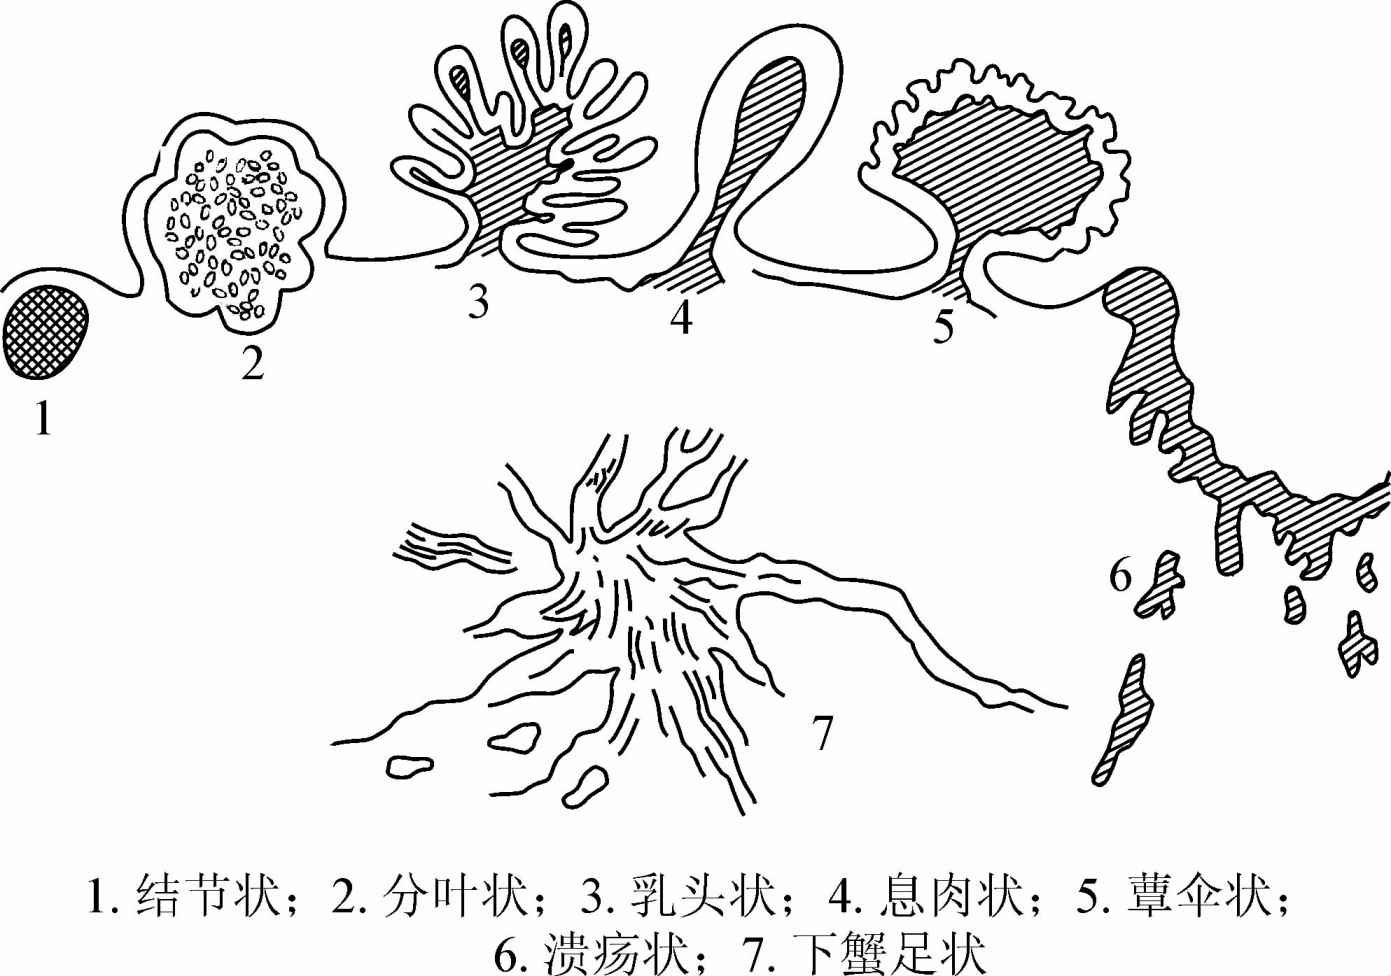
\includegraphics[width=0.5\textwidth]{./images/Image00068.jpg}
  \caption{肿瘤的大体(模式图)}
  \label{fig5-1}
\end{figure}

\subsubsection{肿瘤的大小}

肿瘤的大小相差悬殊,与其良恶性、生长时间、发生部位有一定关系。肿瘤早期往往体积较小,有的甚至在显微镜下才能发现。生长在体表、腹膜腔、盆腔的肿瘤可以长得较大,重达数千克,甚至几十千克,如背部脂肪瘤、盆腔的卵巢囊腺瘤。恶性肿瘤生长迅速,较早危及患者生命,因此,体积一般不会太大。生长在颅内、椎管内、声带等处的肿瘤,因发展空间有限,体积一般亦不会太大。长得特别大的肿瘤,多为生长在非要害部位的良性肿瘤。

\subsubsection{肿瘤的数目}

肿瘤大多为单个,少数可呈多个,如子宫多发性平滑肌瘤。有时同一个体不同部位同时或先后出现两种或两种以上原发性恶性肿瘤,称为多原发癌。

\subsubsection{肿瘤的颜色}

肿瘤一般与其起源组织颜色相同,多数呈灰白或灰红。富于血管的血管瘤或内分泌肿瘤呈灰红或暗红色,黑色素瘤呈棕褐色或黑色,脂肪瘤呈淡黄色,分泌黏液的肿瘤呈灰白半透明状。据此,有时可对肿瘤来源作一初步估计。

\subsubsection{肿瘤的硬度}

肿瘤的硬度取决于来源组织、实质和间质的比例及有无变性坏死。肿瘤中如钙盐较多,骨质形成、纤维成分多则质硬。反之当这些成分少,肿瘤细胞多或有出血、囊性变者则质较软。

\subsection{肿瘤的组织结构}

肿瘤的组织结构多种多样,但任何肿瘤在显微镜下都由实质和间质组成,两者有密切的关系。

\paragraph{肿瘤的实质(parenchyma)}
肿瘤的实质是肿瘤细胞的总称,是肿瘤的主要成分,决定肿瘤的性质和起源。根据肿瘤的实质可作出肿瘤的命名、分类和病理诊断。一种肿瘤通常只有一种实质,少数肿瘤可含两种或多种实质成分。

\paragraph{肿瘤的间质(mesenchyma,stroma)}
主要由结缔组织(纤维、基质)和血管组成,有时可有淋巴管和少数残存的神经纤维。肿瘤间质在不同肿瘤中基本相同,无特异性,它对肿瘤细胞起着营养、支持作用。间质中纤维组织丰富的肿瘤质地较硬,反之则较软。血管丰富的肿瘤往往生长较快,反之则较慢。恶性肿瘤细胞还可释放肿瘤血管形成因子,刺激间质毛细血管增生,促进肿瘤生长,而且同恶性肿瘤的浸润和转移有密切关系。此外,间质中常可见数量不等的淋巴细胞、巨噬细胞和浆细胞等浸润。一般来说,间质中炎细胞的浸润起着抗肿瘤的协同作用,限制肿瘤的生长,体现宿主对肿瘤的免疫反应。间质中有大量淋巴细胞、巨噬细胞浸润者较无浸润者预后好,如乳腺的髓样癌和不典型髓样癌。但是研究发现,炎细胞具有两面性,其所释放的部分炎症介质可能促进肿瘤生长和扩散。

\section{肿瘤的异型性}

肿瘤组织在细胞形态和组织结构上,都与其来源的正常组织有不同程度的差异,这种差异称为异型性(atypia)。异型性的大小可用肿瘤组织分化成熟的程度来表示。分化(differentiation)在胚胎学中指原始幼稚细胞在胚胎发育过程中,向不同方向演化趋于成熟的程度。病理学将此术语引用过来,指肿瘤细胞与其发生部位成熟细胞的相似程度。肿瘤细胞异型性小,表示它和正常来源组织相似,分化程度高,则恶性程度低。反之,肿瘤细胞异型性大,和正常来源组织相似性小,肿瘤细胞分化程度低,往往其恶性程度高。异型性是判断良、恶性肿瘤的重要组织学依据。间变(anaplasia)在现代病理学中指肿瘤细胞缺乏分化的状态。由未分化细胞构成的恶性肿瘤称间变性肿瘤。间变性肿瘤多为高度恶性的肿瘤。

\subsection{肿瘤组织结构的异型性}

肿瘤组织结构的异型性是指肿瘤实质和间质的关系紊乱,失去相应正常组织的结构和层次。良性肿瘤组织结构与其来源组织相似,较易判断其起源。例如肠腺瘤的腺体较丰富,腺腔可扩张,腺腔大小不一,但瘤细胞排列整齐。恶性肿瘤的组织结构异型性明显,细胞排列紊乱,失去正常的层次和结构。例如肠腺癌的腺体大小不一,形态十分不规则,甚至不形成腺腔,排列紊乱,腺上皮细胞排列紧密或呈多层(图\ref{fig5-2})。

\begin{figure}[!htbp]
  \centering
  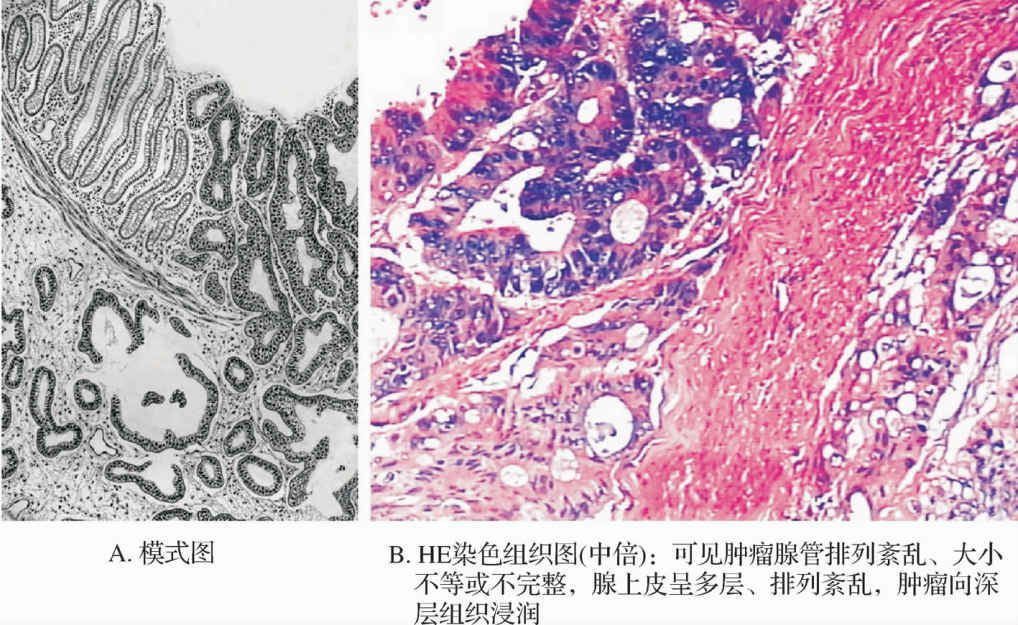
\includegraphics[width=0.68\textwidth]{./images/Image00069.jpg}
  \caption{恶性肿瘤的组织学异型性}
  \label{fig5-2}
\end{figure}

\subsection{肿瘤细胞的异型性}

良性肿瘤细胞异型性小,与其来源的正常细胞相似,有时单从细胞学上无法同其来源的正常细胞区别,其异型性主要表现在组织学方面。恶性肿瘤的瘤细胞具明显的异型性,表现为:

\paragraph{肿瘤细胞的多形性}
表现为瘤细胞大小不一,形态不规则,甚至出现胞体特大的瘤巨细胞。少数分化差的肿瘤细胞较相应组织的正常细胞小,圆形,且大小较一致。

\paragraph{核的多形性}
细胞核大小不一,形态不规则,甚至出现多核、巨核、畸形核瘤细胞。肿瘤细胞核明显增大,因而使核/浆比例增大,从正常的1∶4~6增至1∶1.5~2,甚至1∶1。核染色质呈粗大颗粒状,分布不匀,常靠近核膜分布,使核膜显得增厚。核仁肥大,数目增多。核分裂像多见,并可出现病理性核分裂,即多极性、不对称性、顿挫性核分裂(图\ref{fig5-3},图\ref{fig5-4})。恶性肿瘤细胞核多形性与染色体呈多倍体或非整倍体有关。以上这些改变均有助于病理诊断。

\begin{figure}[!htbp]
  \centering
  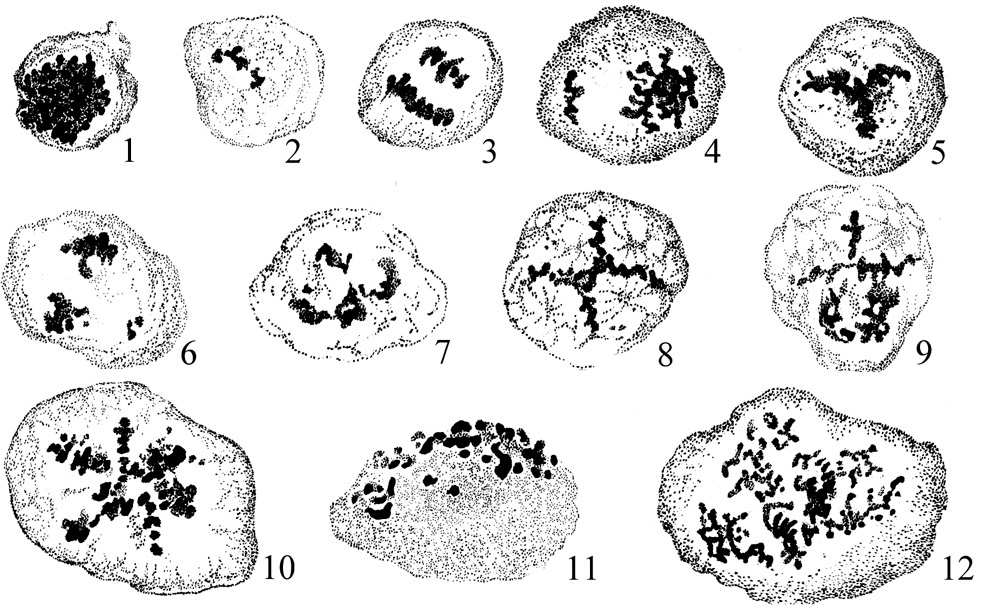
\includegraphics{./images/Image00070.jpg}
  \caption{恶性肿瘤细胞的病理性核分裂像}
  \label{fig5-3}
\end{figure}

\begin{figure}[!htbp]
  \centering
  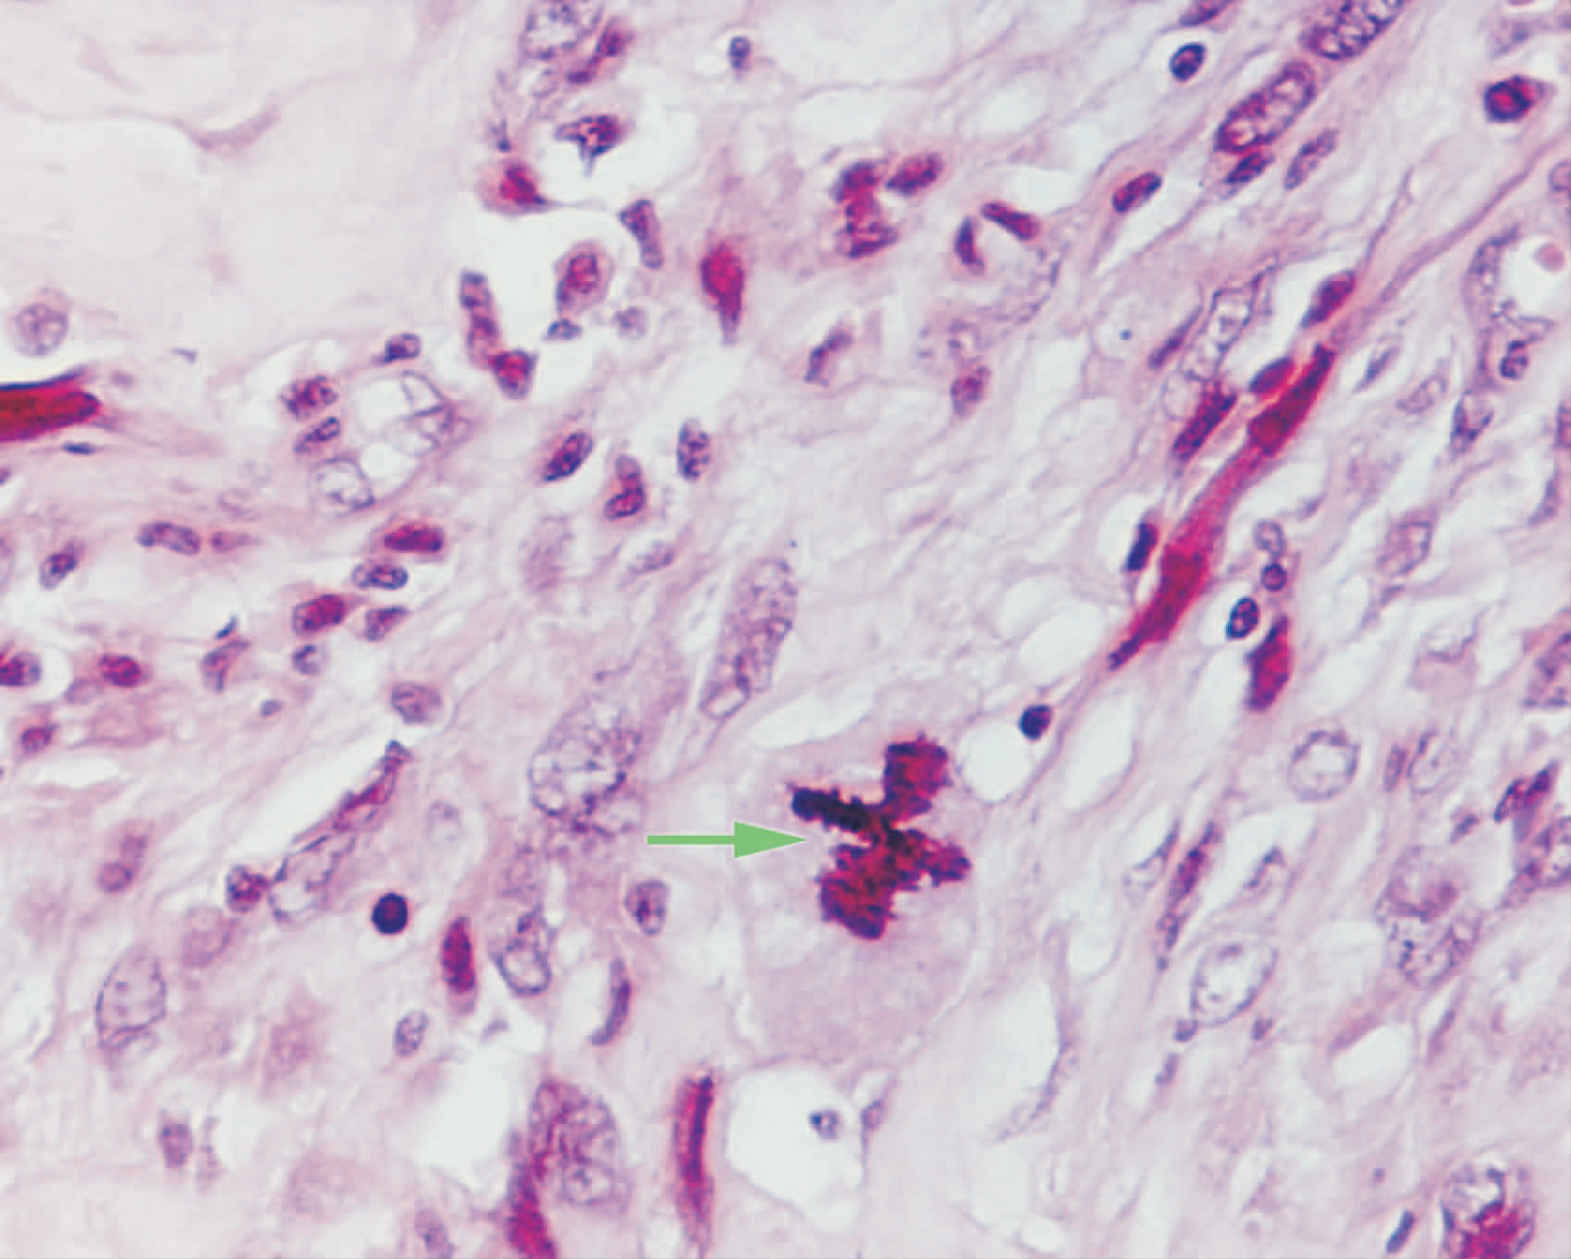
\includegraphics{./images/Image00071.jpg}
  \captionsetup{justification=centering}
  \caption{恶性肿瘤的细胞异型性\\{\small (恶性纤维组织细胞瘤,HE染色,高倍)\\
  瘤细胞大小不一,可见多极病理性核分裂像(箭头所示)}}
  \label{fig5-4}
\end{figure}



\paragraph{胞质的改变}
恶性肿瘤细胞的胞质一般由于分化低而减少,但有时也可以增多。由于胞质内核蛋白体增多,故多呈嗜碱性染色。有些肿瘤细胞内尚可出现黏液、糖原、脂质、色素等肿瘤分泌、代谢产物,并可作为肿瘤鉴别诊断的依据。

\subsection{肿瘤超微结构的异型性}

肿瘤细胞同正常细胞之间或良、恶性肿瘤细胞间未发现有质的差别,而仅有量的差别。主要有以下几个特点:

\paragraph{同型性}
即肿瘤细胞与其来源的正常组织的细胞在超微结构上有相似之处。如鳞状细胞癌有张力原纤维、桥粒,从而有助于诊断。

\paragraph{低分化性}
恶性肿瘤细胞分化程度较低,甚至未分化,如有些横纹肌肉瘤分化低,光镜不见横纹,电镜下可见原始肌节,从而得以确诊。

\paragraph{异型性}
瘤细胞特别是恶性肿瘤细胞、胞核、细胞器显示一定程度的畸形。一般而言,瘤细胞分化越低,细胞器越简单,包括线粒体、内质网、高尔基器、张力微丝等数量减少,发育不良。如鳞癌细胞之间桥粒减少,使瘤细胞易脱落、浸润。又如瘤细胞线粒体呈球形,而非杆状,线粒体嵴呈纵向平行排列,说明其无氧酵解供能的特点。

总的说来,鉴别肿瘤的良、恶性主要靠光学显微镜,而电镜则对鉴别肿瘤的类型和组织来源发挥重要作用。

\subsection{肿瘤细胞的代谢特点}

同正常细胞比,肿瘤细胞的核酸合成代谢明显增强,分解代谢减弱,有利细胞分裂和增殖。其糖代谢在有氧或无氧条件下,均以糖酵解过程占优势,该特性可能与线粒体功能障碍有关。肿瘤的蛋白质合成、分解与代谢均增强,合成代谢又超过分解代谢,并可夺取正常组织营养,这是造成恶病质的重要原因之一。肿瘤还可合成肿瘤蛋白,作为肿瘤特异抗原和相关抗原,引起机体免疫反应。有的肿瘤蛋白与胚胎组织有共同抗原性,称为肿瘤胚胎性抗原,如肝细胞癌能合成胎儿肝细胞所产生的甲种胎儿蛋白(AFP),又如大肠癌可产生癌胚抗原(CEA),临床上检测这些抗原有助于诊断相应的肿瘤和判断疗效。肿瘤的酶代谢活性多数无改变,少数情况表现酶活性增高,如前列腺癌患者酸性磷酸酶(ACP)增高,肝癌、骨肉瘤患者碱性磷酸酶(AKP)活性增高,临床血清学检查可作为辅助诊断。在一些细胞分化原始幼稚者,其酶变化特点主要表现为特殊功能酶接近或完全消失,从而导致酶谱的一致性,同胚胎细胞的酶谱相似。

\section{肿瘤的生长与扩散}

\subsection{肿瘤的生长}

\subsubsection{肿瘤的生长方式}

\paragraph{膨胀性生长}
为多数良性肿瘤的生长方式。良性肿瘤生长缓慢,随着肿瘤体积逐渐增大,推挤周围正常组织呈结节状生长,常有完整的包膜,同周围组织分界清楚,易于手术摘除,术后不易复发(图\ref{fig5-5}A)。

\paragraph{浸润性生长}
为多数恶性肿瘤的生长方式。肿瘤侵入周围组织间隙,浸润破坏周围组织,犹如树根长入泥土一样,因而肿瘤无包膜,与正常组织无明显界限(图\ref{fig5-5}B)。触诊时,肿瘤固定不动,手术不易切除干净,术后易复发,要加放疗、化疗消灭残留的瘤细胞。

关于恶性肿瘤浸润性生长机制,研究颇多,主要有关因素为:瘤细胞具有旺盛的增殖能力,内部压力加大,促使其侵入周围间隙;瘤细胞附着器官后即伸出伪足,以阿米巴样运动侵入,电镜发现伪足中有丰富的微丝;瘤细胞间黏着力下降,可能与瘤细胞膜钙离子含量减少和细胞间连接装置不发达有关;瘤细胞释放溶解酶,溶解周围正常组织,有利于恶性肿瘤细胞的浸润。

\paragraph{外生性生长}
体表、体腔或自然管道表面的肿瘤,常向表面生长,形成突起的乳头状、息肉状、蕈伞状新生物(图\ref{fig5-5}C)。外生性生长可见于良性肿瘤,也可见于恶性肿瘤,但恶性肿瘤在外生性生长的同时还有基底部的浸润性生长,形成基底部浸润性肿块。

\begin{figure}[!htbp]
  \centering
  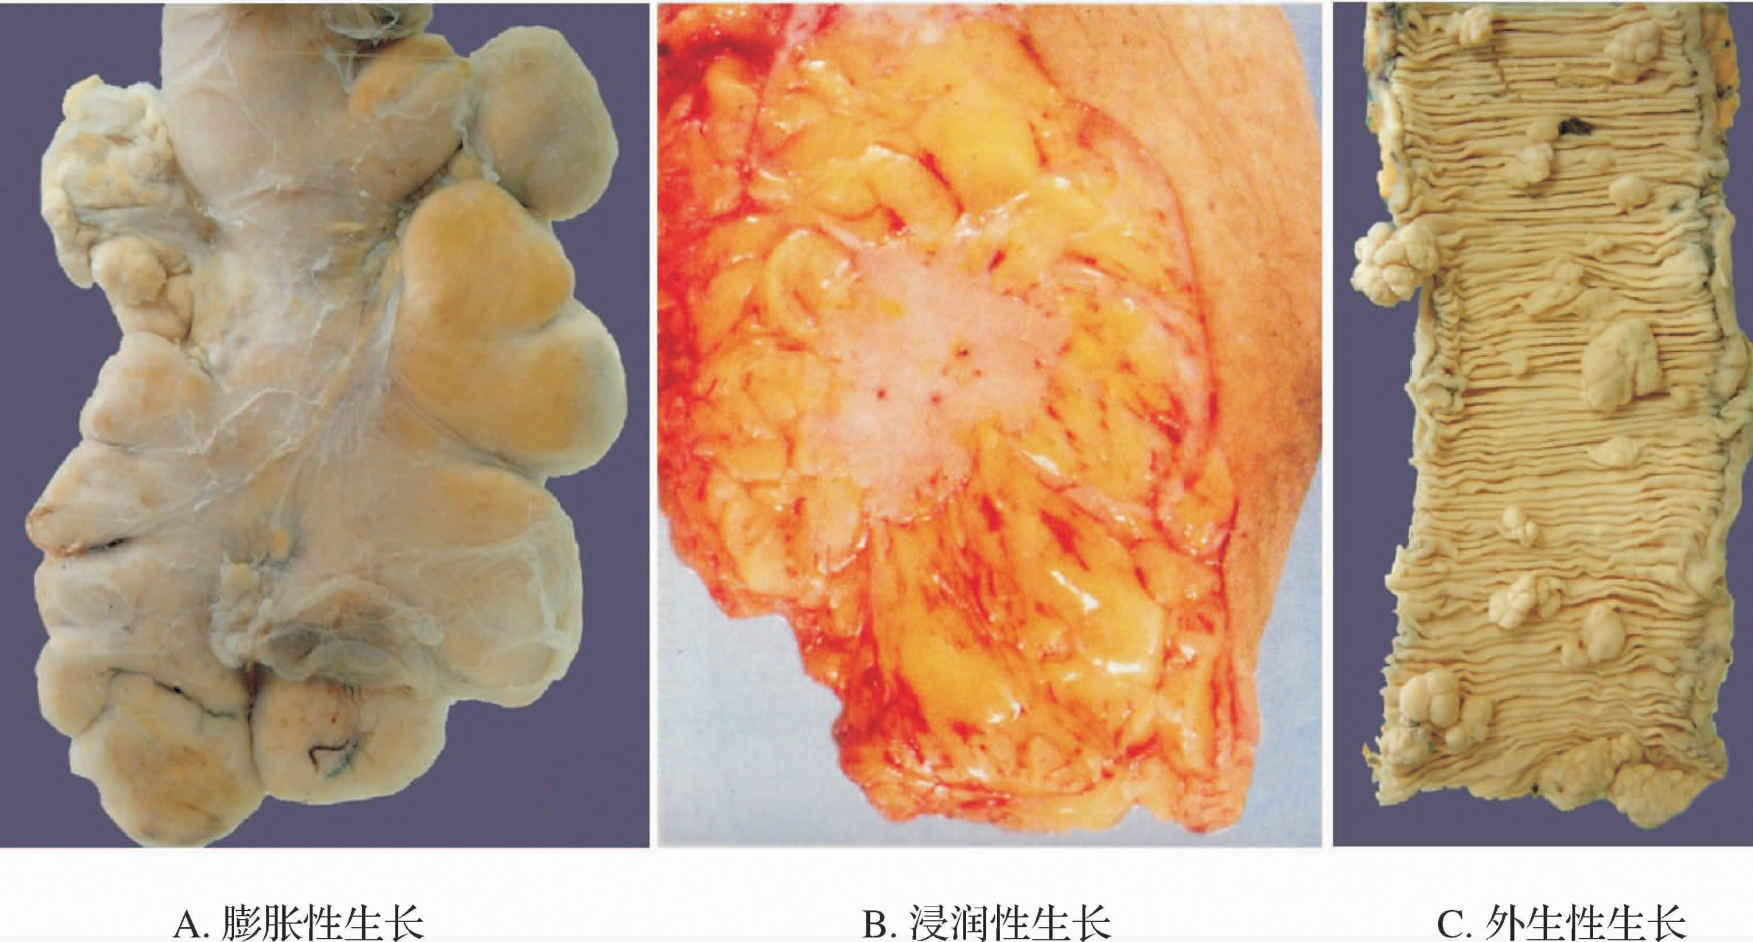
\includegraphics[width=0.66\textwidth]{./images/Image00072.jpg}
  \caption{肿瘤生长方式}
  \label{fig5-5}
\end{figure}

\subsubsection{肿瘤生长动力学}

肿瘤细胞有别于正常细胞的重要表现之一是它们能持续地生长。良性肿瘤分化程度高,生长缓慢,而恶性肿瘤,特别是那些分化程度甚低的肿瘤,其生长速度快,短期内就可形成巨大肿块。生长缓慢的良性肿瘤若生长速度突然加快或体积迅速增大可能为恶性变,但有时亦可为肿瘤继发性出血、坏死及囊性变造成的假象,如甲状腺腺瘤出血囊性变。肿瘤的生长速度与以下三个因素有关:

\paragraph{肿瘤细胞倍增时间(doubling time)}
过去认为,恶性肿瘤生长迅速与肿瘤倍增时间缩短有关。目前实验发现,多数恶性肿瘤细胞的倍增时间与正常细胞相似或者更长。因此恶性肿瘤的生长速度快并不是由于其细胞倍增时间缩短造成的。

\paragraph{生长分数(growth fraction)}
生长分数指肿瘤细胞群体中处于增殖阶段(S期+G{2}
期)细胞的比例。显然生长分数越高肿瘤生长速度越快。在细胞恶性转化的初期,绝大多数的细胞处于复制期,所以生长分数很高。但是随着肿瘤的持续生长,不断有瘤细胞发生分化,离开增殖阶段的细胞越来越多,使得大多数肿瘤细胞处于G{0}
期。即使是生长迅速的肿瘤,如小细胞肺癌,其生长分数也只在20%左右。

\paragraph{瘤细胞的生成与丢失}
瘤细胞的生成大于丢失导致肿瘤不断长大。由于营养供应不足、坏死脱落以及机体抗肿瘤反应等因素的影响,有相当一部分瘤细胞失去生命力,在形态学上表现为凋亡。

综上所述,肿瘤的生长速度取决于生长分数和肿瘤细胞的生成和丢失之比,而与倍增时间关系不大。肿瘤细胞动力学的知识在肿瘤的化学治疗上有重要意义。目前几乎所有的抗癌药物均针对处于增殖期的细胞。因此高生长分数的肿瘤(如高度恶性的淋巴瘤为40%)对于化学治疗特别敏感;而常见的实体瘤(如结肠癌)生长分数低(约5%),故对化学治疗不够敏感。临床上治疗这些肿瘤的战略是先用放射或手术治疗将肿瘤缩小或去除,让残存的瘤细胞从G{0}
期进入增殖期后再用化学治疗。

\subsubsection{肿瘤血管生成}

血液供应是决定肿瘤生长速度最重要的外部条件。临床与动物实验都证明,如果没有新生血管形成来供应营养,肿瘤在达到1~2
mm的直径或厚度后(约10{7}
个细胞)将不再增大。因此诱导血管生成的能力是恶性肿瘤能生长、浸润与转移的前提之一。肿瘤刺激宿主血管持续生长,为其供应营养的过程叫做肿瘤血管形成(angiogenesis)。研究发现,肿瘤细胞及炎细胞能产生血管生成因子,如血管内皮生长因子(vascular
endothelial growth
factor,VEGF),诱导新生血管的生成。目前,抑制肿瘤血管生成正成为一个治疗肿瘤的新途径。

\begin{center}
  \textbf{知识链接}
\end{center}
\chapterabstract{1999年美国Maniotis等根据对人眼葡萄膜黑色素瘤微循环的研究,首次提出了一种与经典肿瘤血管生成途径不同,不依赖机体内皮细胞的全新肿瘤微循环模式,即血管生成拟态(vasculogenic
mimicry,VM)的概念。VM的提出对以内皮依赖性血管是肿瘤微循环唯一方式的传统观念提出了挑战,同时也是对肿瘤血管生成理论的重要补充。VM的形态特点为:肿瘤组织PAS染色可见相互连接成环状的网络通道,这些PAS阳性管道与周边的正常血管联系紧密,且部分管道呈vWF、CD34和VEGFR-2等内皮细胞标记物染色阳性。在透射电镜下,可见血管通道由内衬的薄层基板构成血管壁,但没有内皮细胞。基板上可见侵袭性强和失去分化能力的肿瘤细胞,管腔里面可观察到红细胞。}

\subsubsection{演进和异质性}

肿瘤的演进(progression)指恶性肿瘤在生长过程中变得越来越富有侵袭性的现象,包括生长加快、浸润周围组织和远处转移等。肿瘤的异质性(heterogeneity)指肿瘤细胞的不同亚克隆在侵袭能力、生长速度、对生长信号的反应、对药物敏感性等方面的差异。

\subsection{肿瘤的扩散}

肿瘤的扩散是恶性肿瘤的重要特征之一,肿瘤的扩散有直接蔓延和转移两种方式。

\subsubsection{局部浸润和直接蔓延}

肿瘤细胞连续不断地沿着组织间隙、淋巴管、血管、神经束衣等侵入和破坏邻近正常组织或器官,并继续生长称做直接蔓延(direct
spread)。例如晚期子宫颈癌可蔓延侵及膀胱、直肠、阴道壁及盆腔组织。

肿瘤局部浸润和直接蔓延的机制比较复杂,大致可分为四个步骤:①癌细胞表面黏附分子减少:正常上皮细胞表面有各种黏附分子,它们之间的相互作用,有助于使细胞黏附在一起,阻止细胞移动。肿瘤细胞表面黏附分子减少,使细胞彼此分离;②癌细胞与基底膜的黏着增加:正常上皮细胞与基底膜的附着是通过上皮细胞基底面的一些分子介导的,如层粘连蛋白受体。癌细胞有更多的层粘连蛋白受体,并分布于癌细胞的整个表面,使癌细胞与基底膜的黏着增加;③细胞外基质的降解:癌细胞产生蛋白酶,溶解细胞外基质成分,使基底膜产生局部缺损,让癌细胞通过;④癌细胞迁移:癌细胞借阿米巴样运动通过基底膜缺损处移出。癌细胞穿过基底膜后,进一步溶解间质结缔组织,在间质中移动。到达血管壁时,又以相似的方式穿过血管的基底膜进入血管。

\subsubsection{转移(metastasis)}

恶性肿瘤的瘤细胞从原发部位侵入淋巴管、血管或体腔,被带到它处继续生长,形成同原发瘤同样类型的肿瘤,这个过程称做转移。所形成的肿瘤称做继发瘤或转移瘤。良性肿瘤不转移,恶性肿瘤常有转移。一般来说,恶性肿瘤分化程度越低,浸润性越强,转移率越高。转移这一过程的完成至少包括三个基本步骤:①侵入:瘤细胞侵入局部淋巴管、血管、体腔或自然管道。②管腔内转运:瘤细胞随淋巴液、血液或腔道运送至他处。③停驻和增殖:瘤细胞停驻下来,在新的部位增殖,形成与原发瘤同样组织类型的肿瘤。影响恶性肿瘤转移的因素很多,包括瘤细胞本身、局部血液供应、生化环境(如甲状腺、胰腺不利于生长)、组织或器官结构功能(脾血窦、肌肉收缩不利于转移)及全身免疫状况等。常见的转移途径有以下三种。

(1)淋巴道转移:淋巴道是癌最常见的转移途径,即瘤细胞侵入淋巴管,随淋巴液到达局部淋巴结,停留下来生长形成转移瘤(图\ref{fig5-6},图\ref{fig5-7})。如甲状腺癌转移到颈部淋巴结,阴茎癌转移至腹股沟淋巴结,乳腺外上象限区的乳腺癌首先到达同侧腋窝淋巴结,其中肿瘤原发部位淋巴液引流的第一站淋巴结称前哨淋巴结,对前哨淋巴结的活检有助于判断是否有淋巴结转移。转移至淋巴结的癌细胞首先到达被膜下边缘窦,以后累及整个淋巴结,使淋巴结肿大、质较硬,切面灰白色。淋巴道转移一般由近到远,但有时会越过引流淋巴结而累及更下一站的淋巴结,即“跳跃性转移”,也可逆流至附近淋巴结群引起转移。了解肿瘤的淋巴道转移规律,有助于发现原发瘤,有助于采取合理治疗措施及提示预后,如胃癌若发生左锁骨上淋巴结转移,则提示肿瘤已发生广泛转移和预后不良。

\begin{figure}[!htbp]
  \centering
  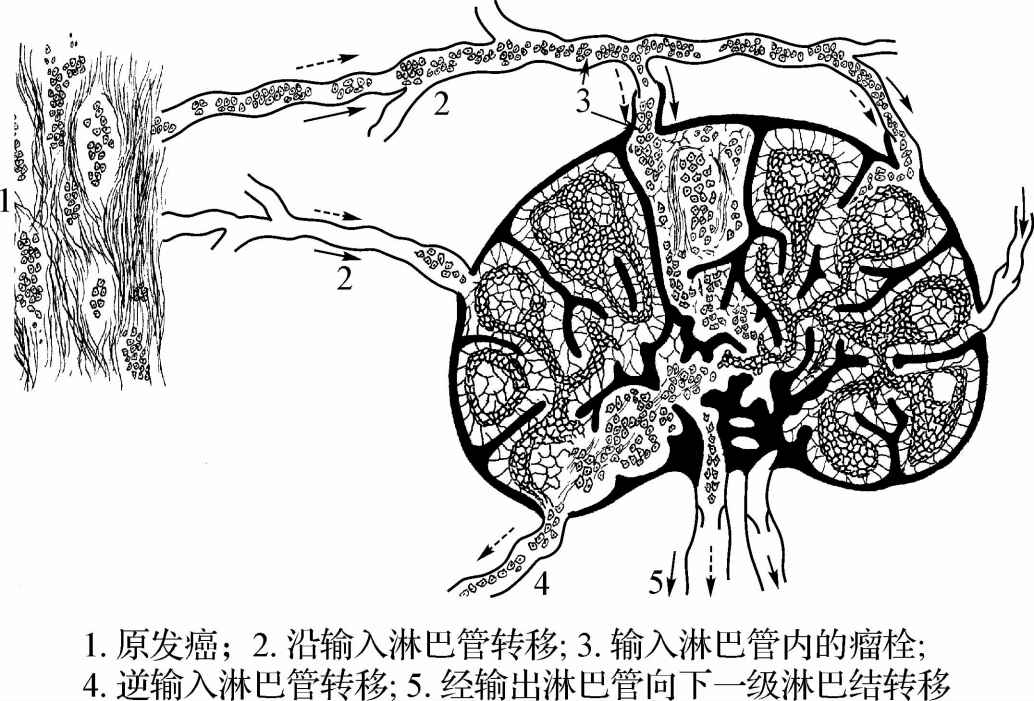
\includegraphics[width=0.6\textwidth]{./images/Image00073.jpg}
  \caption{恶性肿瘤经淋巴道转移的模式图}
  \label{fig5-6}
\end{figure}

\begin{figure}[!htbp]
  \centering
  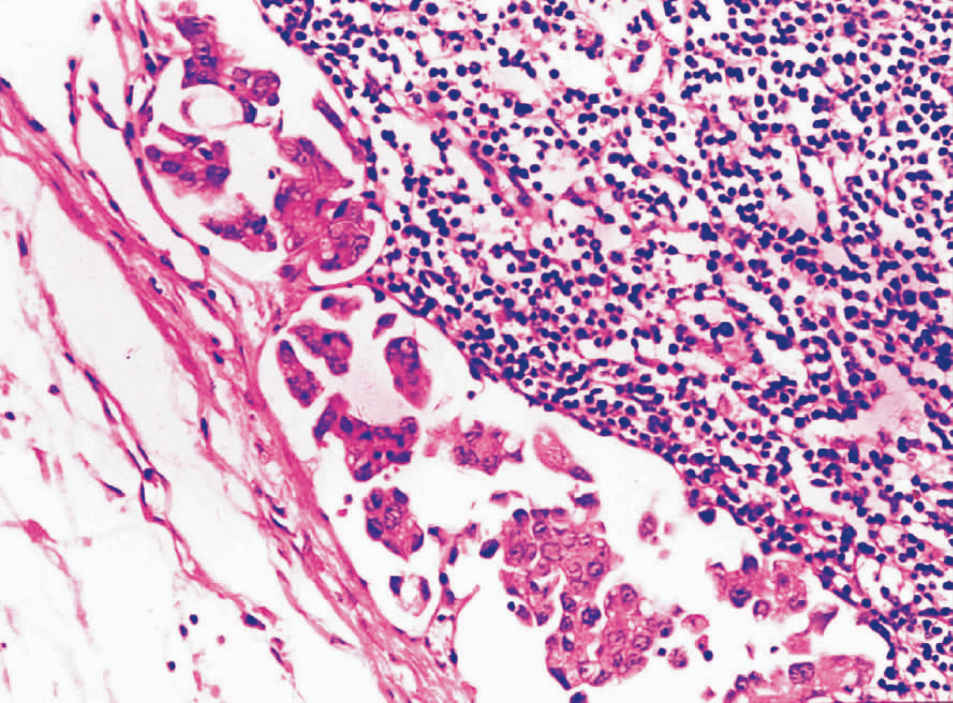
\includegraphics[width=0.5\textwidth]{./images/Image00074.jpg}
  \caption{淋巴结转移癌(HE染色,中倍)\\ {\small 淋巴结被膜下边缘窦内为转移的癌组织}}
  \label{fig5-7}
\end{figure}



(2)血道转移:恶性肿瘤细胞侵入血管后,随血流到达远隔器官继续生长,形成转移瘤。肉瘤组织血管丰富,瘤细胞弥散分布与血管关系密切,故血道转移是肉瘤最常见的转移方式。此外,未分化癌和癌的晚期也可发生血道转移。瘤细胞主要侵入壁薄、管内压力较低的毛细血管和小静脉内,少数也可经淋巴管入血。进入血流的瘤细胞,以瘤栓的形式随血流方向运行而阻塞在被滞留的部位,瘤细胞在此增殖,然后穿出血管壁形成转移瘤。

血道转移的运行途径与血栓栓塞的运行过程相似,一般情况下与血管解剖部位及血流方向有关。侵入体静脉系统的瘤细胞多经右心到肺,引起肺转移;肝接受门静系统的血液,故胃肠道肿瘤易于经门静脉引起肝转移;侵入肺静脉的瘤细胞,经左心进入主动脉系统,形成全身器官的广泛转移;侵入胸、腰、骨盆静脉的瘤细胞可经吻合支进入椎静脉系统,引起椎骨及中枢神经系统的转移,如前列腺癌可以没有肺转移而发生椎管的转移。少数情况下,当静脉回流受阻(如咳嗽引起腹腔内压增高),可发生逆行性转移。

血道转移性肿瘤常为多发性散在分布的圆球形结节,边缘较整齐。位于器官表面的转移瘤,中央部位常因缺血坏死而塌陷,形成所谓“癌脐”(图\ref{fig5-8}),有助于同原发瘤区别。由于肺、肝为最易发生转移瘤的器官,所以在诊断肿瘤或肿瘤病人手术前,必须仔细检查肝和肺。

(3)种植性转移:体腔内器官的肿瘤蔓延至器官浆膜面时,瘤细胞可脱落下来,像播种一样种植在体腔浆膜的表面,形成许多转移瘤,这种转移方式称为种植性转移(图\ref{fig5-9})。胸膜或腹膜腔内肿瘤的瘤细胞脱落后可种植到肋膈角、直肠膀胱陷窝、膀胱子宫陷窝等处。晚期胃癌可致双侧卵巢表面种植性转移,称作克鲁根勃瘤(Krukenberg
tumor)。脑、脊髓肿瘤可经脑脊髓腔种植于颅底、脊髓背侧和马尾等处。

浆膜腔的种植性转移,可致下列后果:由于浆膜下淋巴管或毛细血管被癌栓阻塞,或由于小血管受损通透性增加与破裂,引起浆液性或血性积液,抽取积液涂片寻找恶性瘤细胞有助于诊断;有时胃肠、卵巢等处的黏液腺癌转移可致大量黏液积聚,称之为“腹膜假黏液瘤”;瘤细胞浸润使浆膜面相互融合或纤维蛋白渗出导致机化,使浆膜面粘连,引起肠梗阻等后果。

\begin{figure}[!htbp]
  \centering
  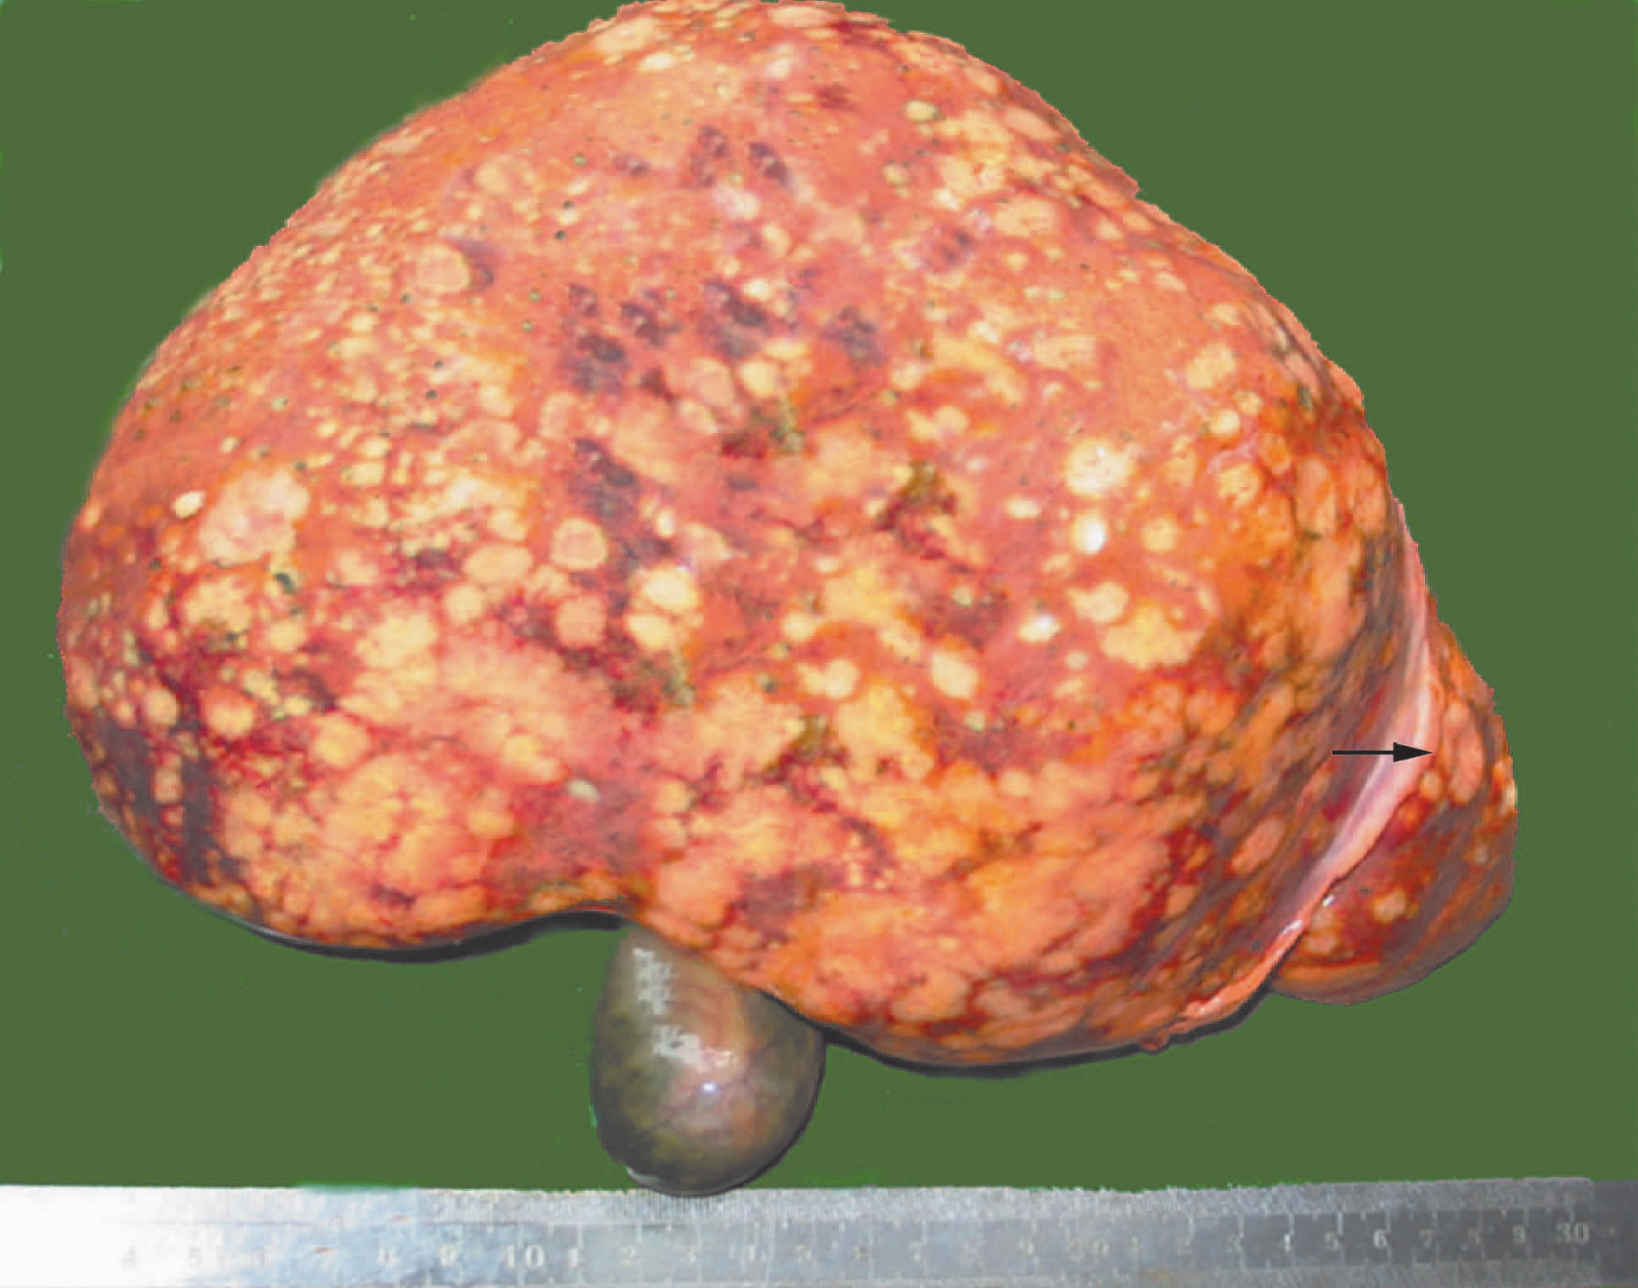
\includegraphics{./images/Image00075.jpg}
  \caption{肝转移性胃癌 \\ {\small 肝脏表面满布瘤结节,可见癌脐(箭头所示)}}
  \label{fig5-8}
\end{figure}



\begin{figure}[!htbp]
  \centering
  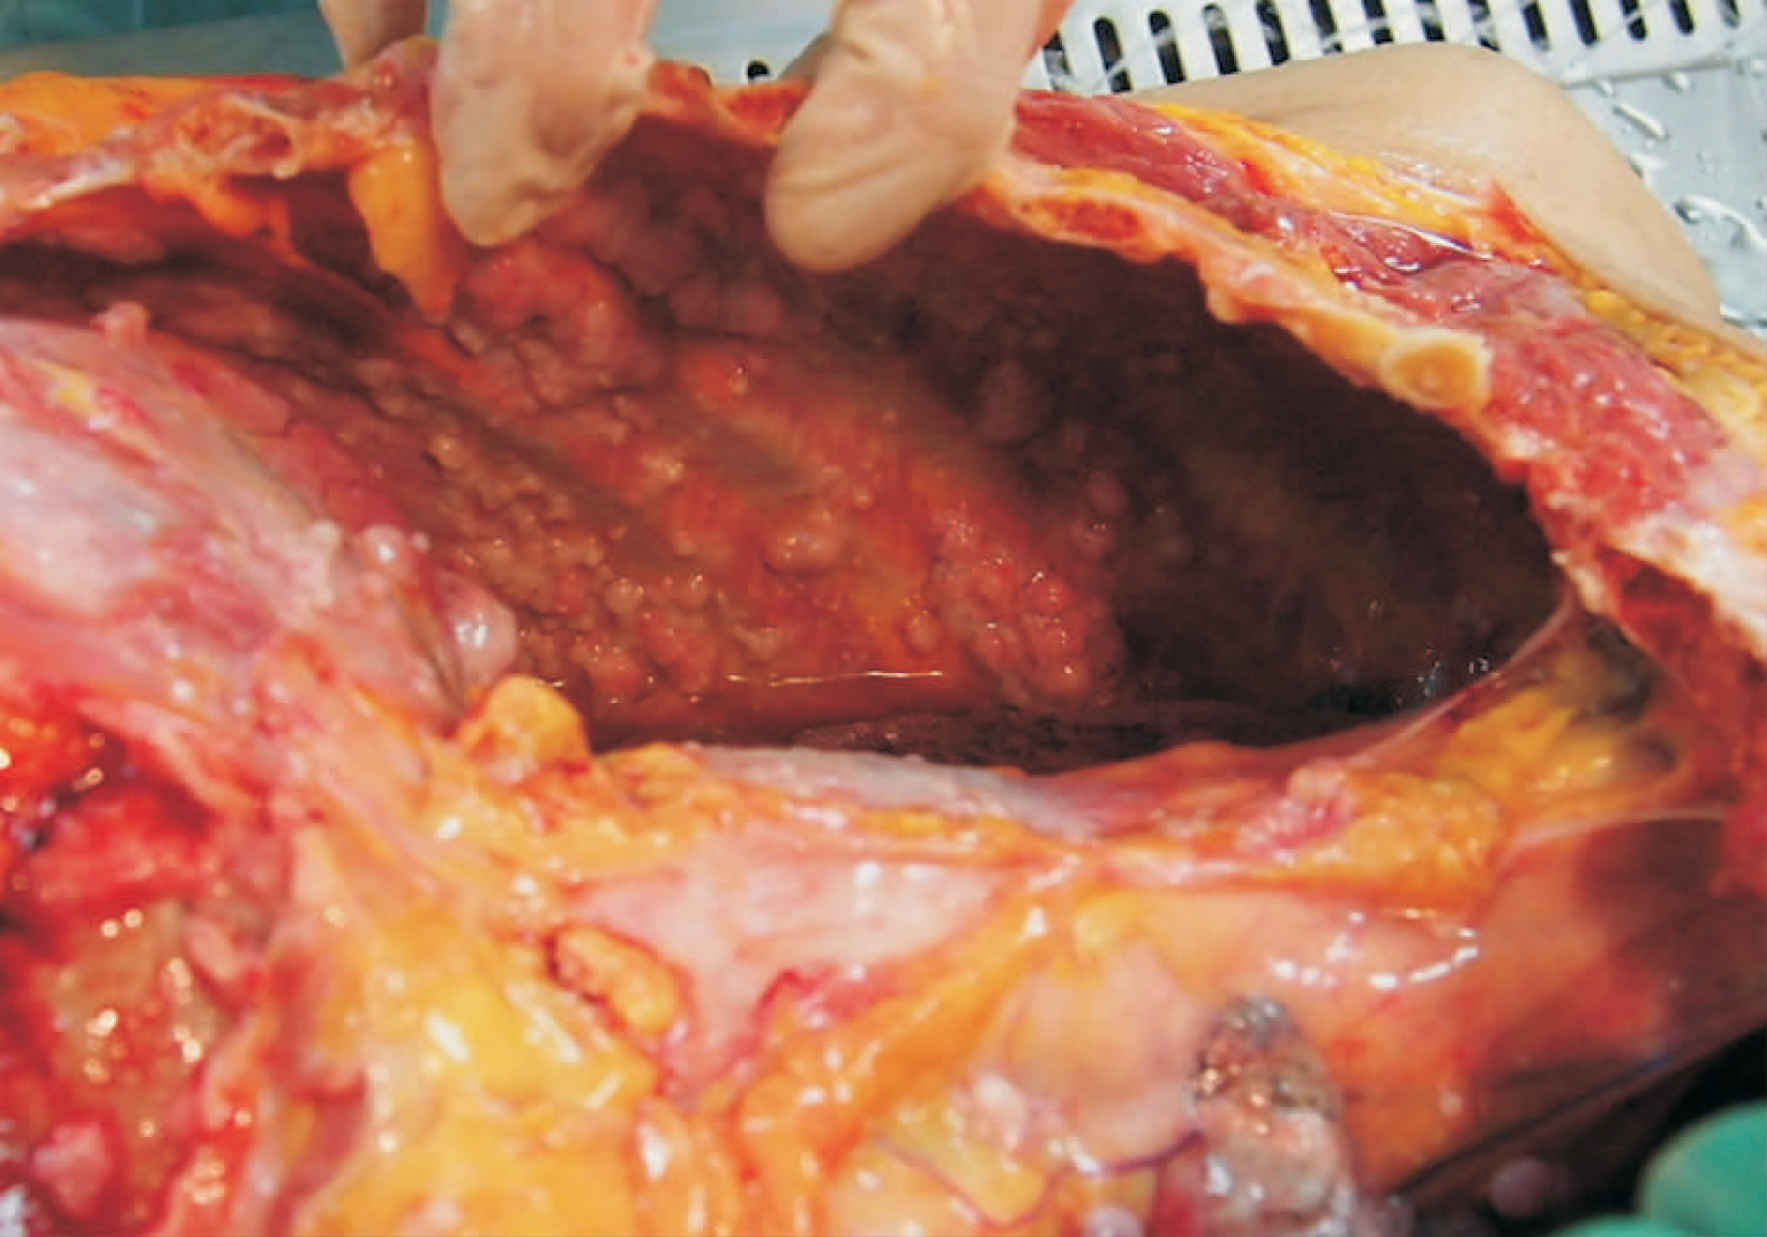
\includegraphics{./images/Image00076.jpg}
  \caption{胸膜壁层转移性卵巢癌 \\ {\small 胸膜表面布满大小不等瘤结节,此为卵巢癌种植性转移}}
  \label{fig5-9}
\end{figure}



种植性转移在少数情况也可为医源性的,见于外科手术时,肿瘤细胞沾染了手术野,引起手术切口等处种植性转移。

\subsubsection{原发瘤和转移瘤的鉴别}

在临床病理工作中,鉴别原发瘤和继发瘤十分重要,有时相当困难,需要综合临床、病理、免疫病理等资料,作出较为准确的诊断。

\paragraph{病史}
多数情况下,身体两个以上部位的肿瘤,先出现者为原发瘤,后出现者为转移瘤。

\paragraph{数目}
原发瘤常为单个,转移瘤常为多个。但应注意肝、肺的原发瘤也可呈多结节状,肺的转移性恶性肿瘤也可呈单个结节。

\paragraph{癌周组织}
癌巢附近的组织对鉴别有参考价值。如颈部、皮下癌组织旁见到残余的淋巴组织,则有利于转移癌的诊断,乳腺癌伴有囊性增生等则有利于原发癌的诊断。

\paragraph{癌组织的形态和结构}
转移瘤多保持原发瘤的形态结构特点。但部分转移瘤可因微环境的改变与原发瘤在形态上不尽一致,如部分胃腺癌分化程度低,不形成腺腔,但转移灶中可出现明显腺腔。

\paragraph{部位}
肝与肺的多发性瘤结节常是转移瘤。肺的转移瘤多来自肾、肝、子宫和乳腺等的各种癌或肉瘤。肺癌常转移至肝、肾上腺、骨和脑等。骨的转移瘤多来自甲状腺、前列腺和肾。乳腺癌易转移到肾上腺、卵巢等处。

\paragraph{免疫病理和电镜检查}
有时据上述方法仍无法判别原发瘤和继发瘤,则可根据肿瘤的特点,进行免疫标记或电镜观察等加以确诊。

\subsection{肿瘤的复发}

肿瘤的复发指肿瘤经外科手术切除或放射治疗后,临床上获得过一段治愈期或缓解期后又重新出现同样的肿瘤。复发性肿瘤可发生在原部位、相邻部位或远隔部位。引起肿瘤复发的原因可为肿瘤细胞残留,如因肿瘤的浸润性生长,手术难以切除干净。亦可为隐性转移灶的存在,当机体免疫机能下降时,转移灶瘤细胞增殖形成临床上所见的肿块。肿瘤的复发主要见于恶性肿瘤,但有些良性肿瘤,如腮腺多形性腺瘤、血管瘤、韧带样纤维瘤,由于它们与周围组织分界不清难以切除干净,故易复发。少数良性肿瘤多次复发后还可恶变。

\subsection{肿瘤的分级与分期}

\subsubsection{肿瘤的分级}

肿瘤的分级(grading of
tumor)是根据肿瘤细胞分化程度的高低、异型性的大小及核分裂像的多少来确定恶性程度的级别。分级方法从两级分级法(低级别和高级别)至四级分级法,在临床病理工作中都有所应用,不同的肿瘤有不同的分级方法。

\subsubsection{肿瘤的分期}

肿瘤的分期(staging of
tumor)是根据肿瘤的大小范围、浸润深度和转移的程度来确定肿瘤病程发展的早晚。目前常用的有国际抗癌组织(UICC-Union
International Control
Cancer)的TNM系统(图\ref{fig5-10}),即根据肿瘤的范围(T{1~4}
),淋巴结有否转移及转移情况(N{0~3} ),远处转移的有无(M{0~1}
)给予定期。此外还有美国癌分期联合学会(AJCS-American Joint Committee on
Cancer
Staging)的肿瘤分期法,即据肿瘤的范围(原位、器官内、器官外、侵入邻近器官、远处转移)将肿瘤分为五期,该分期法临床更为实用。

\begin{figure}[!htbp]
  \centering
  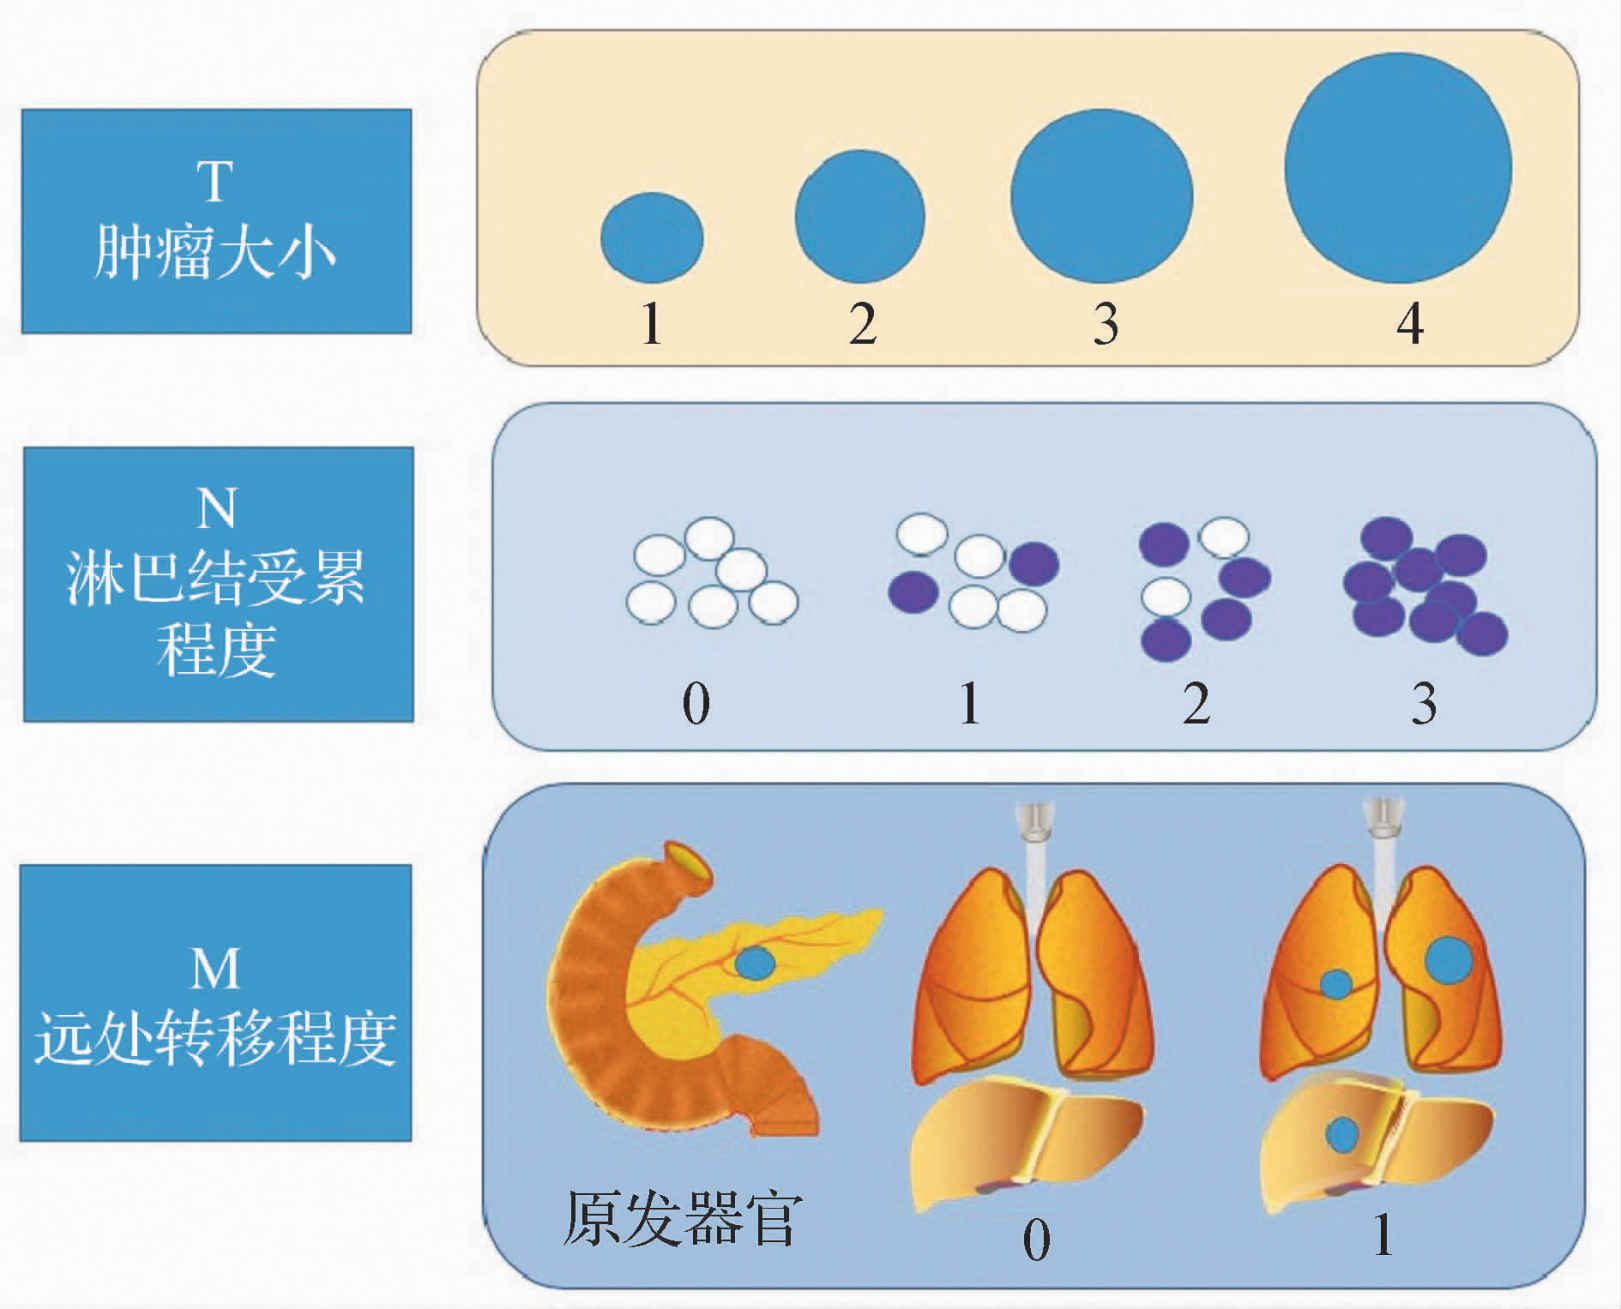
\includegraphics{./images/Image00077.jpg}
  \caption{肿瘤分期示意图}
  \label{fig5-10}
\end{figure}

\section{肿瘤对机体的影响}

\subsection{良性肿瘤对机体的影响}

良性肿瘤由于分化成熟,生长缓慢,总的来说对机体影响较小,主要对周围器官产生压迫和阻塞作用,一般无致命后果。如几十千克的卵巢囊腺瘤患者可长期带瘤生存,但生长在颅内或椎管内的良性肿瘤可引起颅内压增高或脊髓受压,产生相应的神经系统症状。肾上腺的嗜铬细胞瘤,可引起阵发性高血压,胰岛细胞瘤可引起阵发性低血糖,分泌生长激素的垂体腺瘤可引起巨人症和肢端肥大症。另外,良性肿瘤若产生并发症,后果也是严重的。如卵巢囊腺瘤可发生蒂扭转(图\ref{fig5-11}),使瘤体出血坏死,必须紧急手术处理。少部分良性肿瘤可恶性变,一般为多发性或易复发的良性肿瘤,如肠多发性息肉病中的一半患者可恶变为腺癌;膀胱移行上皮乳头状瘤易恶变为移行上皮癌。

\begin{figure}[!htbp]
  \centering
  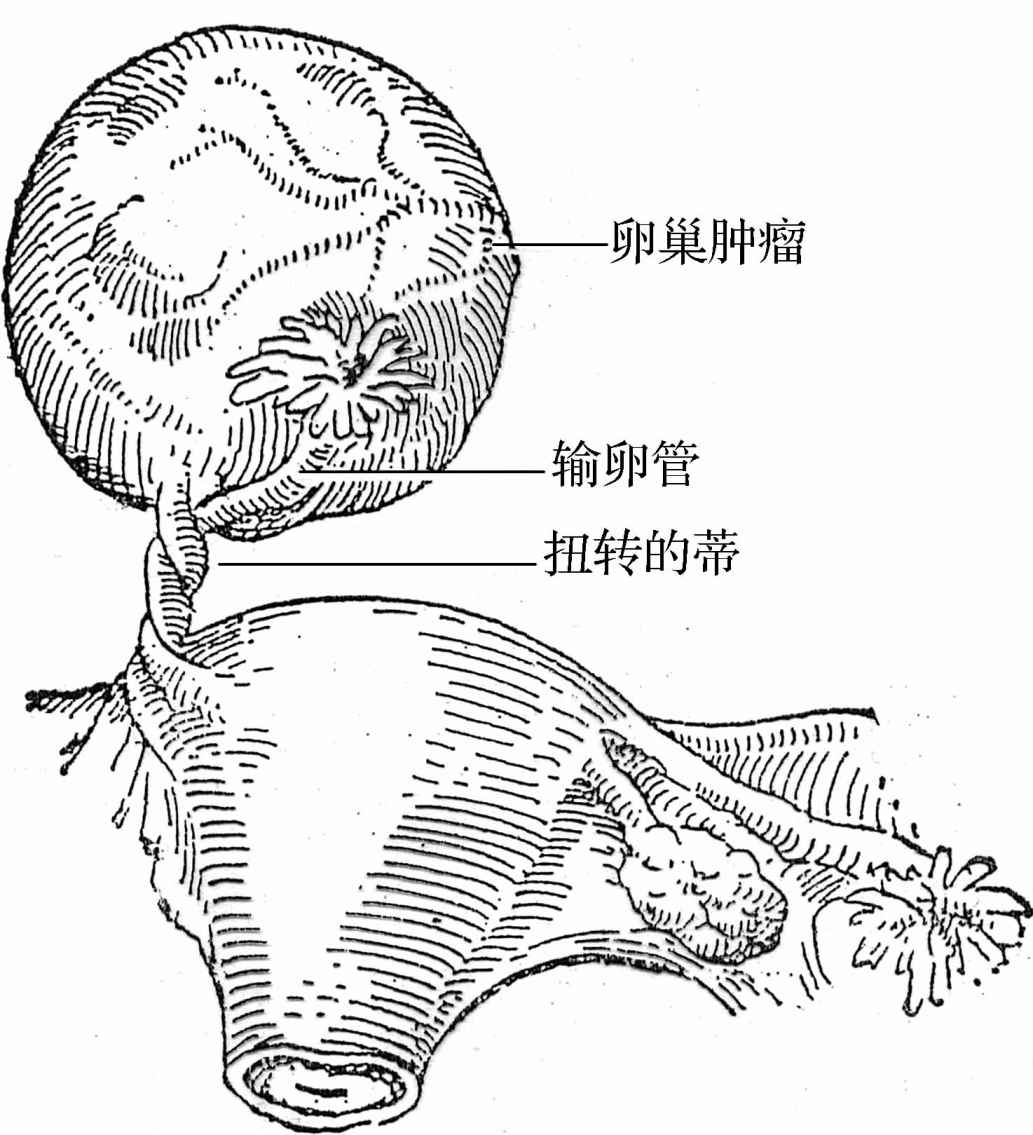
\includegraphics[scale=1.2]{./images/Image00078.jpg}
  \caption{卵巢肿瘤蒂扭转}
  \label{fig5-11}
\end{figure}

\subsection{恶性肿瘤对机体的影响}

恶性肿瘤由于分化不成熟,生长较快,浸润破坏组织器官,发生远处转移,并常引起出血、坏死、溃疡、穿孔和感染等继发性改变,对机体影响较大,后果更为严重。除上述良性肿瘤对机体的影响外,恶性肿瘤尚有下述影响:

\subsubsection{浸润和转移}

常常是恶性肿瘤致死的主要原因,如癌的脑转移。

\subsubsection{发热}

恶性肿瘤常可引起发热,多为肿瘤代谢产物、坏死组织毒性产物或合并感染所致。

\subsubsection{副肿瘤综合征}

一些来自非内分泌腺肿瘤也可产生激素或激素样物质(异位激素),引起相应症状和体征,称为异位内分泌综合征。如支气管燕麦细胞癌、胸腺瘤、淋巴瘤等可产生抗利尿激素,葡萄胎、睾丸胚胎癌、前列腺癌等可产生促甲状腺素等。产生异位激素的肿瘤称为异位内分泌肿瘤,多见于癌,但也可见于肉瘤如纤维肉瘤、平滑肌肉瘤等。除上述异位内分泌综合征外,肿瘤患者还可出现一些原因不明的临床表现(常由肿瘤产物、异常免疫反应等引起),包括神经、肌肉、皮肤、骨关节、软组织、造血及肾损伤等,上述异常临床综合征统称副肿瘤综合征(paraneoplastic
syndrome)。

\subsubsection{恶病质(cachexia)}

恶病质指由于恶性肿瘤或其他慢性消耗性疾病导致机体严重消瘦、贫血、虚弱、全身衰竭的状态(图\ref{fig5-12})。恶病质多见于晚期恶性肿瘤患者。有些肿瘤如食管癌,因梗阻进食困难,恶病质出现较早。恶病质发生机制为诸因素综合作用所致,包括精神因素、肿瘤生长消耗大量营养物质、肿瘤代谢产物堆积引起机体代谢紊乱、食欲下降、失眠、疼痛、出血、感染等。

\begin{figure}[!htbp]
  \centering
  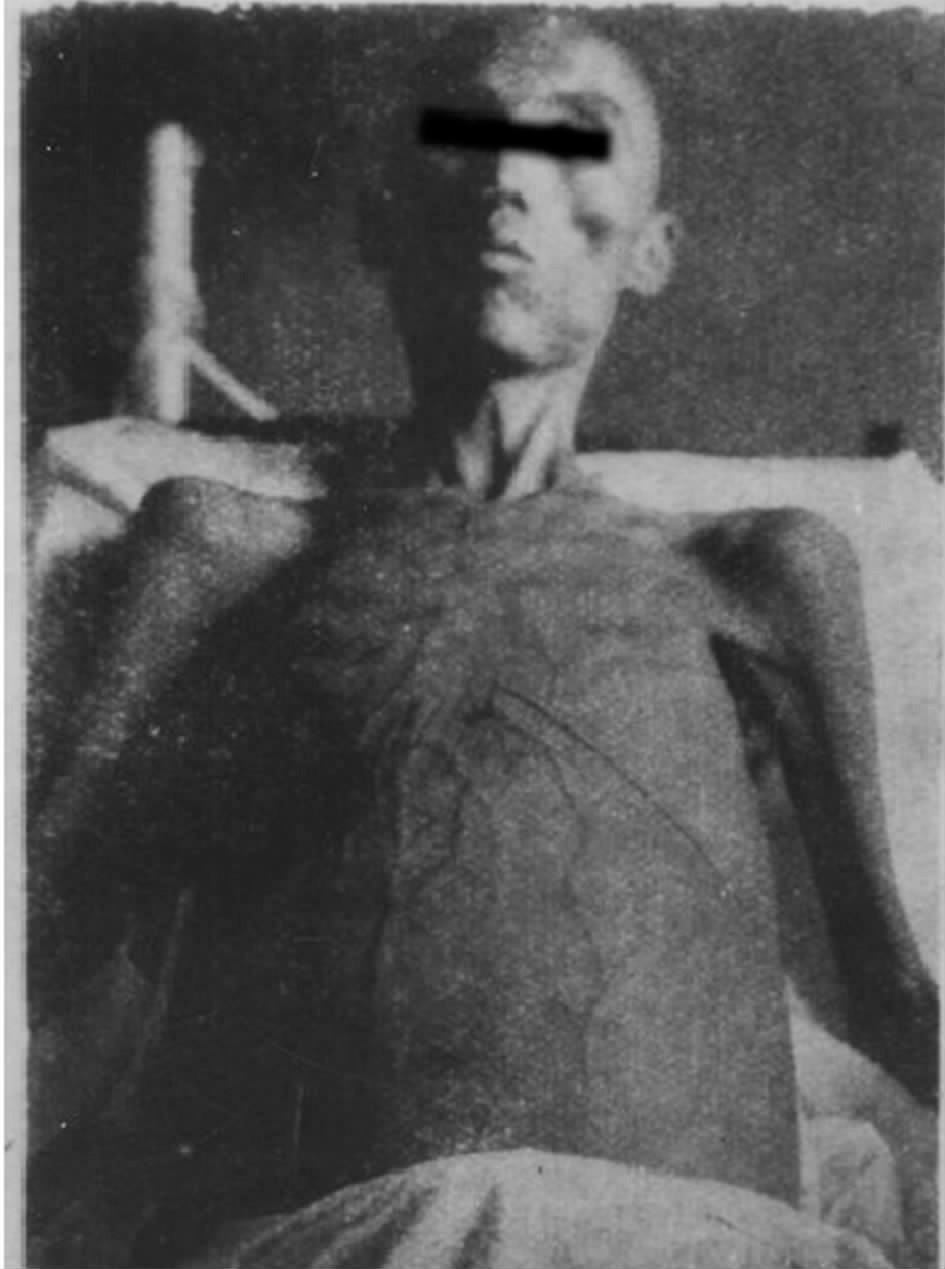
\includegraphics{./images/Image00079.jpg}
  \caption{恶病质 \\ {\small 原发性肝癌晚期患者,极度消瘦、衰弱}}
  \label{fig5-12}
\end{figure}



\section{良性肿瘤与恶性肿瘤的区别}

根据肿瘤的分化程度、生物学行为及对机体的危害程度等将其分为良性肿瘤和恶性肿瘤。区别良性肿瘤和恶性肿瘤,对于正确诊断和治疗具有重要的实际意义,肿瘤的良恶性区别见表\ref{tab5-3}。

\begin{table}[ht]
  \caption{良性肿瘤与恶性肿瘤的区别}
  \label{tab5-3}
  \centering
  \begin{tabular}{lp{5cm}p{5cm}}
    \toprule
                 & 良性肿瘤                                                           & 恶性肿瘤                                          \\
    \midrule
    组织分化程度 & 分化好,异型性小                                                   & 分化不好,异型性大                                \\
    核分裂       & 无或稀少,无病理性核分裂像                                         & 多见,可见病理性核分裂像                           \\
    生长速度     & 缓慢                                                               & 较快                                              \\
    生长方式     & 膨胀性和外生性生长,前者常有包膜,同周围组织一般分界清楚,常可推动 &
    浸润性和外生性生长,前者无包膜,同周围组织分界不清,不易推动,后者同时伴有浸润性生长                                                   \\
    继发改变     & 很少出血、坏死                                                     & 常有出血、坏死、溃疡                              \\
    转移         & 不转移                                                             & 常有转移                                          \\
    复发         & 很少复发                                                           & 较多复发                                          \\
    对机体影响   & 较小,主要为局部压迫、阻塞                                         & 较大除压迫阻塞外还可引起出血,合并感染,甚至恶病质 \\
    \bottomrule
  \end{tabular}
\end{table}

判断良恶性肿瘤的根据是多方面的,转移是判断良恶性最重要的标准。一个肿瘤只要发生了转移,即使异型性很小,都属恶性肿瘤,如甲状腺滤泡性腺癌有时异型性并不大,却发生了转移。而又有一些良性肿瘤,如非典型性纤维黄色瘤,虽有瘤细胞的异型性,却没有浸润转移。可见肿瘤的形态学表现和生物学行为有时并非一致。另外,良性肿瘤也可发生恶变,如肠腺瘤性息肉可恶变为肠腺癌。罕见情况下,有些恶性肿瘤可转化为良性肿瘤,如神经母细胞瘤转变为节细胞性神经瘤。

良性肿瘤与恶性肿瘤之间无绝对界限。还有一些肿瘤不能截然划分为良性、恶性,而需要根据其形态特点评估其复发转移的风险度(低、中、高)。肿瘤从良性到恶性之间还存在交界性肿瘤(borderline
tumor),即指组织形态和生物学行为介于良性与恶性之间,有恶变倾向的一类肿瘤。如卵巢交界性浆液性乳头状囊腺瘤,在一定条件下可向恶性发展,转变为浆液性乳头状囊腺癌。认识交界性肿瘤,以便临床上进行适度的积极治疗和随访工作。

\section{常见肿瘤举例}

\subsection{上皮性肿瘤}

\subsubsection{良性上皮性肿瘤}

\paragraph{乳头状瘤(papilloma)}
由被覆上皮发生,向表面呈乳头状增生,乳头中央为纤维结缔组织和血管组成的轴心(图\ref{fig5-13})。乳头表面被覆增生的上皮因部位不同,可为分化成熟的鳞状上皮、柱状上皮或移行上皮。乳头状瘤的间质和上皮(实质)如同手指和手套的关系。瘤细胞分化好,无浸润现象,常见于皮肤、口腔黏膜、鼻、鼻窦、喉头、外耳道、膀胱等。发生在外耳道、膀胱、阴茎及喉部的乳头状瘤手术后易复发,其中部分可转变为乳头状癌。

\begin{figure}[!htbp]
  \centering
  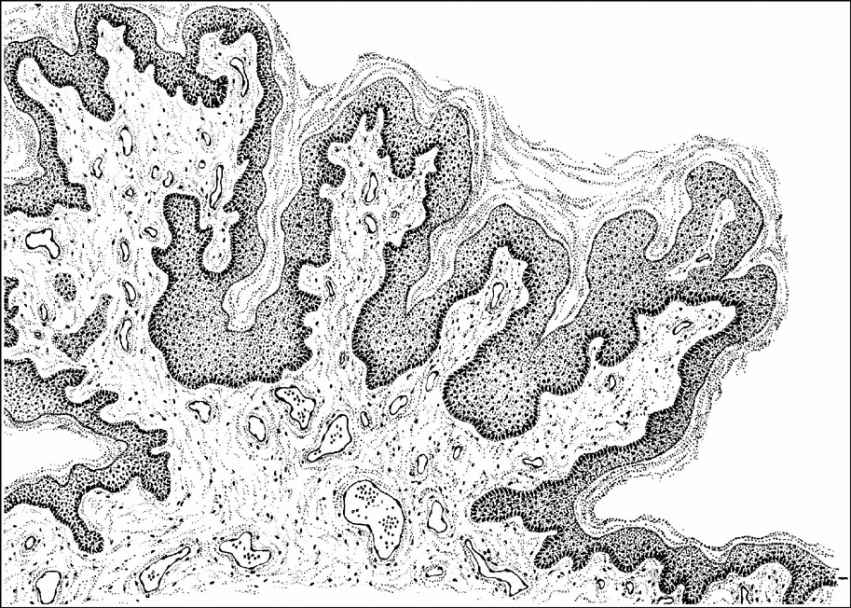
\includegraphics{./images/Image00081.jpg}
  \caption{皮肤乳头状瘤\\{\small 乳头表面的瘤细胞与正常鳞状上皮相似,乳头的中央为肿瘤间质}}
  \label{fig5-13}
\end{figure}



\paragraph{腺瘤(adenoma)}
由腺上皮发生,常见于甲状腺、卵巢、乳腺、涎腺和胃肠道,也见于汗腺、皮脂腺、垂体、肾上腺皮质、肾脏等。腺瘤的腺体在结构上与其来源腺体相似,且常具有一定的分泌功能。不同之处在于腺体大小、形态不规则,排列紧密,缺乏典型的小叶和导管,有时腺管扩张成囊肿。较常见的腺瘤类型有:

(1)囊腺瘤:好发于成年女性卵巢,单侧多见,肿瘤呈结节状,切面见大小不等的囊腔。根据腺上皮的不同又可分为:①浆液性囊腺瘤:腺上皮分泌浆液,部分可呈乳头状生长,易发生恶变。②黏液性囊腺瘤:腺上皮分泌黏液,常呈多房性,囊壁光滑,少有乳头状生长。

(2)纤维腺瘤:为年轻妇女乳腺常见的良性肿瘤,多为单个,结节状,境界清楚,有包膜,切面灰白。镜下由增生的腺管及纤维结缔组织共同组成肿瘤的实质。

(3)息肉状腺瘤:多见于结肠。肠黏膜腺上皮增生,呈息肉状,有蒂同肠黏膜相连。多发性者又称结肠多发性息肉病,是一种具有家族倾向的遗传性疾病,可造成肠梗阻,有的早期就可发生癌变。

(4)多形性腺瘤:多发生于唾液腺的闰管和肌上皮。肿瘤由腺体、鳞状上皮、肌上皮、黏液样及软骨样成分构成,形态多样,习惯又称混合瘤。中年人好发,肿瘤呈结节状或分叶状,表面有纤维包膜,该肿瘤较易侵犯包膜,切除后易复发或恶变。

\subsubsection{恶性上皮性肿瘤}

由上皮组织起源的恶性肿瘤称为癌。癌是人类最常见的一类恶性肿瘤,中、老年人好发。癌生长速度较快,以浸润性生长为主,与周围组织界限不清,发生在皮肤、黏膜的癌常呈菜花状、蕈伞状或息肉状,表面常有坏死出血和溃疡形成;发生在器官内的癌常为不规则结节状,呈树根样或蟹足状向周围组织浸润。癌组织因间质较多而质地较硬,切面灰白色、干燥。镜下观:癌细胞紧密排列呈条索状或腺腔样结构,称为癌巢。癌巢与间质分界清楚,网状纤维染色可见网状纤维存在于癌巢周围,而癌细胞之间无网状纤维。癌在早期多经淋巴道转移,一般到晚期才发生血道转移。

癌的几种较常见类型如下:

\paragraph{鳞状细胞癌(squamous cell carcinoma)}
简称鳞癌,常发生于正常被覆鳞状上皮的部位,如皮肤、唇、咽、喉、食管、宫颈、外阴、阴茎等处,但也见于正常没有鳞状上皮被覆的部位,通过鳞状上皮化生、增生和异型增生而发展为鳞癌,如支气管、胆囊、肾盂等处。镜下见癌细胞形成大小不一的团块状或条索状的癌细胞巢,并向真皮或黏膜下浸润。癌巢的最外层癌细胞排列整齐,相当于基底层的细胞,其内可见多边形癌细胞,似棘细胞层。分化高者,细胞间还可见细胞间桥,在癌细胞巢的中央出现同心圆性层状排列的角化物,称为角化珠(keratin
pearl)或癌珠(图\ref{fig5-14})。分化差的鳞癌无角化形成,细胞间桥消失,癌细胞异型性明显,核分裂多见,间质较少。

\begin{figure}[!htbp]
  \centering
  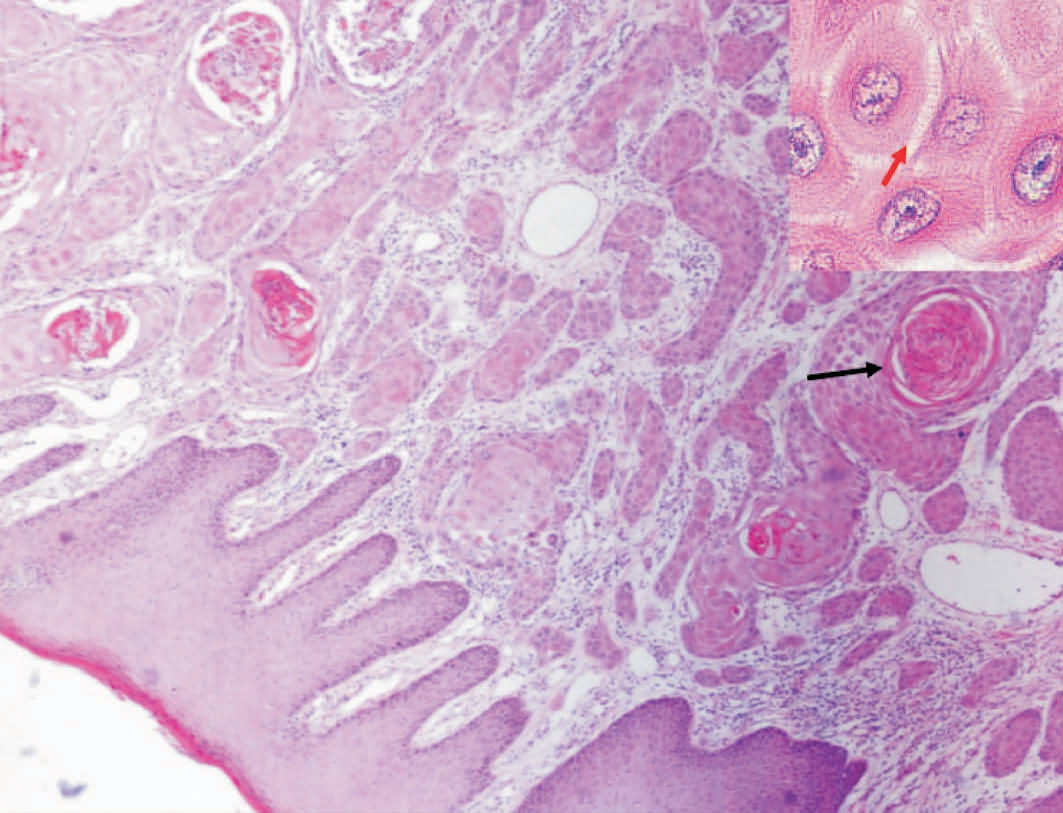
\includegraphics{./images/Image00082.jpg}
  \captionsetup{justification=centering}
  \caption{鳞状细胞癌(HE染色,低倍)\\{\small 图中可见肿瘤细胞排列成巢团状,中央是呈同心圆状结构的角化珠(黑箭头所示);右上小图显示细胞间桥(红箭头所指)}}
  \label{fig5-14}
\end{figure}



\paragraph{基底细胞癌(basal cell carcinoma)}
来自皮肤及皮肤附件的基底细胞,多见于老年人面部,如眼睑、鼻翼、颊部等处,因癌组织常形成边缘不规则的溃疡,故本癌又称鼠咬状溃疡。镜下见癌细胞巢主要由基底细胞样的癌细胞组成。此癌属低度恶性,生长缓慢,很少发生转移,对放射线敏感,预后较好。

\paragraph{尿路上皮癌(urothelial carcinoma)}
由膀胱或肾盂等处的移行上皮发生,膀胱最多见,肾盂次之,输尿管较少发生。肿瘤外形呈乳头状,有蒂,单发或多发。镜下见癌细胞似尿路上皮样多层排列,有不同程度异型性,分化好者形成乳头结构,分化差者不形成乳头,细胞异型明显,广泛浸润膀胱壁。

\paragraph{腺癌(adenocarcinoma)}
由腺上皮、导管上皮及柱状上皮覆盖的黏膜发生的恶性肿瘤,多见于胃肠道、呼吸道、子宫、乳腺、甲状腺、胰腺等组织器官。根据形态结构和分化程度可分为分化较好的具有腺体结构的管状腺癌(图\ref{fig5-15})和乳头状腺癌、以实性癌巢为主要表现的低分化腺癌及分泌黏液较多的黏液腺癌。

\begin{figure}[!htbp]
  \centering
  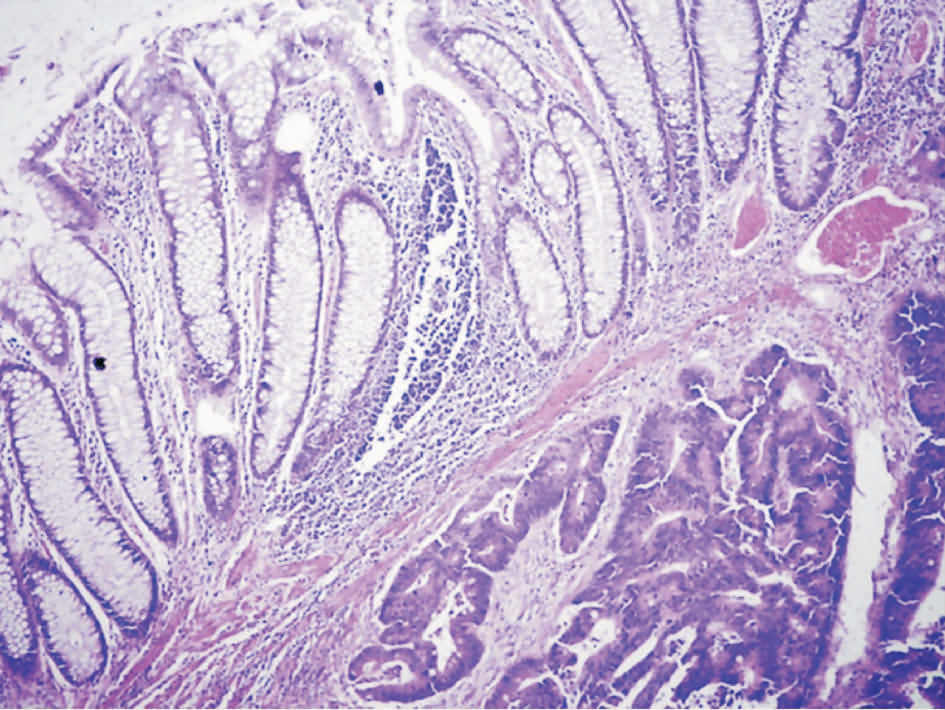
\includegraphics{./images/Image00083.jpg}
  \caption{腺癌(HE染色,低倍)\\{\small 癌细胞形成腺管状结构,与正常腺体相比,有明显的组织结构异性性和细胞异性性}}
  \label{fig5-15}
\end{figure}



(1)管状腺癌(tubular
adenocarcinoma):常见于胃肠、胆囊、子宫体等,肉眼观:肿瘤常呈息肉状、菜花状或结节状,常伴溃疡形成。镜下观:癌细胞呈单层或多层,排列成大小不一、形态多样的腺样结构,瘤细胞核分裂像多见。如腺腔高度扩张呈囊状者,称为囊腺癌。

(2)乳头状腺癌(papillary
adenocarcinoma):腺癌组织内若癌细胞主要排列成乳头状结构时即称为乳头状腺癌。以甲状腺最为多见。如果细胞向囊腔内呈乳头状生长时称为乳头状囊腺癌。

(3)黏液癌(mucoid
carcinoma):主要见于胃肠道,镜下有两种表现:一种为黏液积聚在癌细胞内,并逐渐将核挤向一侧,使癌细胞呈印戒状,当这种印戒样细胞弥漫成片,而腺样结构很少时,称为印戒细胞癌或黏液细胞癌;另一种为癌细胞产生大量细胞外黏液,形成大小不一的“黏液湖”,癌细胞则成堆或散在漂浮在黏液湖中,称为黏液腺癌。黏液癌大体上呈灰白色、湿润、半透明似胶冻,故又称胶样癌。

\paragraph{未分化癌}
来源于上皮组织,分化程度低,难以辨别其来源上皮类型的恶性肿瘤。镜下观:癌细胞呈弥漫分布,多不形成明显巢状结构,细胞异型性大,核分裂像多见,常需同肉瘤加以区别。未分化癌恶性度高,常发生血道转移,预后差,但对放射线和化疗药物敏感。

\subsection{间叶组织肿瘤}

间叶组织肿瘤来源广泛,发病年龄较上皮性肿瘤者轻,良恶性的相对性更为突出。间叶组织可相互转化的特点造成肿瘤成分复杂,形态多样,如纤维瘤中可出现骨成分。肿瘤特点不但与组织发生有关,而且与生长部位有关。

\subsubsection{良性间叶组织肿瘤}

\paragraph{纤维瘤(fibroma)}
由纤维组织发生的良性肿瘤。多见于皮下、肌腱、筋膜等处。常为单发,呈圆形、椭圆形或分叶状,可有或无包膜,边界清楚,质地坚韧。瘤组织由成熟的纤维细胞及成束状排列的胶原纤维组成,间质为血管及少量疏松的结缔组织。纤维瘤生长缓慢,切除后多不复发。

需要指出的是还有组织形态和纤维瘤相似的一大组病变,统称为纤维组织瘤样增生或纤维瘤病(fibromatosis)。常见的有韧带样纤维瘤、瘢痕疙瘩、结节性筋膜炎等。病变特点为纤维组织增生形成瘤样肿块,但并非真性肿瘤。增生的瘤样纤维组织比较成熟,但在局部常呈浸润性生长,无包膜,有时纤维母细胞生长较活跃,细胞丰富,核肥大,甚至具有一定的异型性,如切除不完全,可多次复发,但不转移。此种病损可发生在身体任何部位的软组织,以皮下、筋膜、肌肉为多,尤以四肢及腹壁多见。

\paragraph{脂肪瘤(lipoma)}
是最常见的一种良性肿瘤,多发生于人体躯干和四肢的皮下组织,以颈部和肩背部最常见,腹膜后、胃肠道及肾脏也可发生。大多为单发,也可多发。生长较慢,肉眼观多呈分叶状,质软,有薄的纤维结缔组织包膜与周围组织分界。切面呈黄色,脂肪样。镜下见瘤组织由成熟的脂肪细胞组成,与正常脂肪组织的区别为有完整包膜。脂肪瘤手术易切除。

\paragraph{脉管瘤}
脉管瘤由血管及淋巴管发生,分别称为血管瘤(hemangioma)及淋巴管瘤(lymphangioma),其中以血管瘤较多见。两者均常见于婴儿及儿童,多为先天性脉管组织发育异常,而非真性肿瘤。血管瘤多见于面部、颈部、唇、舌、口腔及肝、脾等内脏器官,常呈紫色或红色,可平坦或隆起于表面,无包膜,与周围界限不清。其组织结构有两种类型:一种系由多数毛细血管密集而成,管腔明显或不明显,称毛细血管瘤;另一种由内皮细胞增生形成大小形状不一的血窦,似海绵状结构而称海绵状血管瘤。两种类型的瘤组织也可混合存在。血管瘤可随身体的发育而长大,成年后即停止发展,甚至可自然消退。

淋巴管瘤常见于唇、舌、颈部及腋下等处。肿瘤呈灰白色,半透明,无包膜,与周围组织境界不清。切面可见多个囊腔,内含淋巴液。发生于颈部的巨大淋巴管瘤,瘤组织内淋巴管扩张呈囊状,称为囊性淋巴管瘤或水瘤。

\paragraph{平滑肌瘤(leiomyoma)}
平滑肌瘤最多见于子宫,其次为胃肠道。肉眼观:肿瘤多为结节状,境界清楚,质地坚实,可有或无包膜,切面常呈编织状或漩涡状。镜下观:见瘤细胞与正常平滑肌细胞相似,由形态较一致的梭形细胞构成编织状排列,核分裂像很少,在细胞形态和组织结构上有时与纤维瘤很相似,但平滑肌瘤细胞的胞浆较红染,核呈长杆状,两端较钝,V.G染色有助于区别,平滑肌纤维呈黄色,而胶原纤维呈红色。

\subsubsection{恶性间叶组织肿瘤}

恶性间叶组织肿瘤统称肉瘤。肉瘤较癌少见,好发于青少年,肉眼观:肿瘤呈结节状或分叶状,可挤压周围组织形成假包膜,或有清楚的边界。由于生长较快肉瘤体积常较大、质软,切面灰红色,均质性,细腻,湿润似鱼肉状,故称肉瘤。镜下观:肉瘤细胞大多弥散排列,不形成细胞巢,与间质界限不清。网状纤维染色可见肉瘤细胞间存在网状纤维。肿瘤间质富于血管,故肉瘤多先由血道转移,这些特点均与癌有所区别(表\ref{tab5-4})。正确区分癌和肉瘤,具有十分重要的临床意义。

\begin{table}[ht]
  \caption{癌与肉瘤的区别}
  \label{tab5-4}
  \centering
  \begin{tabular}{lp{5cm}p{5cm}}
    \toprule
                 & 癌                                        & 肉瘤                                                \\
    \midrule
    组织来源     & 上皮组织                                  & 间叶组织                                            \\
    发病率       & 较常见,约为肉瘤的9倍,多见于40岁以上成人
                 & 较少见,多见于青少年                                                                            \\
    大体特点     & 质较硬、色灰白、较干燥                    & 质软、色灰红、湿润、鱼肉状                          \\
    组织学特点   & 多形成癌巢,实质与间质分界清楚            & 瘤细胞多弥漫分布,实质与间质分界不清,间质内血管丰富 \\
    网状纤维染色 & 网状纤维围绕癌巢,癌细胞间多无网状纤维    & 肉瘤细胞间多有网状纤维                              \\
    免疫组织化学 & 癌细胞表达上皮标记(如细胞角蛋白)        & 肉瘤细胞表达间叶标记(如波形蛋白)                  \\
    转移         & 淋巴道转移为主                            & 血道转移为主                                        \\
    \bottomrule
  \end{tabular}
\end{table}

常见肉瘤列举如下:

\paragraph{纤维肉瘤(fibrosarcoma)}
纤维肉瘤的发生部位与纤维瘤相似,以四肢皮下及深部组织多见。肉眼观:肿瘤呈巨块型或结节状,与周围组织分界清楚,可形成假包膜,切面粉红或灰白均质。镜下观:肿瘤组织由大小不一的梭形或短梭形细胞构成,瘤细胞产生胶原纤维,呈编织状或旋涡状排列(图\ref{fig5-16})。纤维肉瘤的恶性程度不等,既与分化有关,也与生长部位有关,部位表浅者恶性度较低。

\begin{figure}[!htbp]
  \centering
  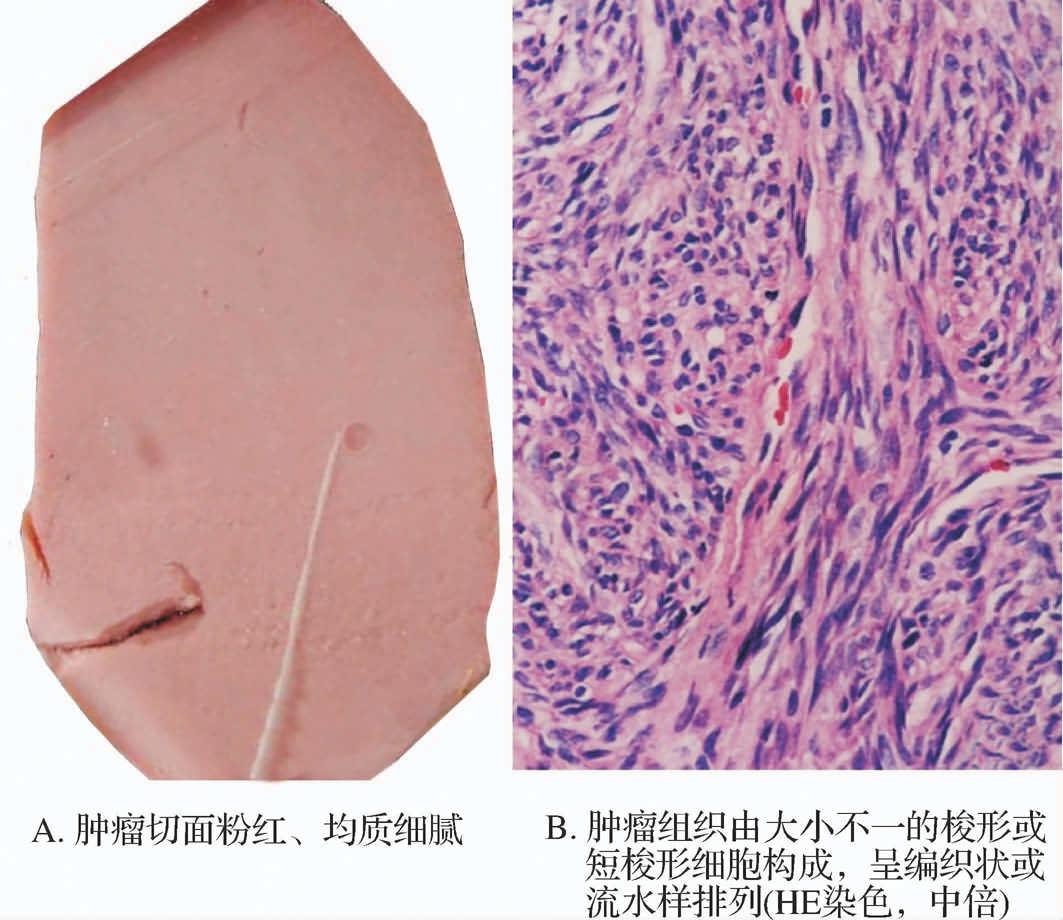
\includegraphics{./images/Image00085.jpg}
  \caption{纤维肉瘤}
  \label{fig5-16}
\end{figure}

\paragraph{脂肪肉瘤(liposarcoma)}
多发生于40岁以上成人,极少见于青少年,是软组织肉瘤中较常见者。多发生于大腿、腘窝、腹膜后,也见于肾周和深部的软组织内。肉眼观:脂肪肉瘤的大体形态差异很大,可似一般的脂肪瘤,也可呈鱼肉状或黏液样外观,大多呈分叶或结节状,表面有假包膜。镜下观:脂肪肉瘤的组织形态多种多样,分化好的其组织结构与脂肪瘤相似,分化差的瘤细胞具有明显的异形性,并有多量的瘤巨细胞。

\paragraph{平滑肌肉瘤(leiomyosarcoma)}
好发于胃肠道和子宫,以中老年多见。肉眼观呈实体性圆形或结节状肿块,边界清楚,部分有假包膜,切面灰红或灰棕色鱼肉状或编织状,较大者可有出血、坏死、囊性变。镜下观:分化好的平滑肌肉瘤同平滑肌瘤较难区分,分化差者瘤细胞具有明显的异型性,核分裂像多见。

\paragraph{骨肉瘤(osteosarcoma)}
是骨组织中最常见、恶性度最高的一种肿瘤,以青年人多见。好发于股骨两端、胫骨上端及肱骨上端,肿瘤起自于干骺端,向髓腔及骨膜下生长,并穿破骨膜,侵入周围软组织,形成放射状新骨,与骨干纵轴垂直或斜行,X线片上形成日光放射状条纹;被瘤组织掀起的骨膜,因有较多骨组织增生,X线片上形成Codman三角,是骨肉瘤的特点。肉眼观:若骨质形成少则呈灰红色鱼肉状,若骨质形成多则较硬。镜下观:瘤细胞高度异型,细胞大小不一、形态不规则,并有瘤巨细胞,核分裂像多见。肿瘤性骨组织的出现是诊断本瘤的组织学依据(图\ref{fig5-17})。本病恶性度极高,发展迅速,早期即可发生血道转移,危及生命。

\begin{figure}[!htbp]
  \centering
  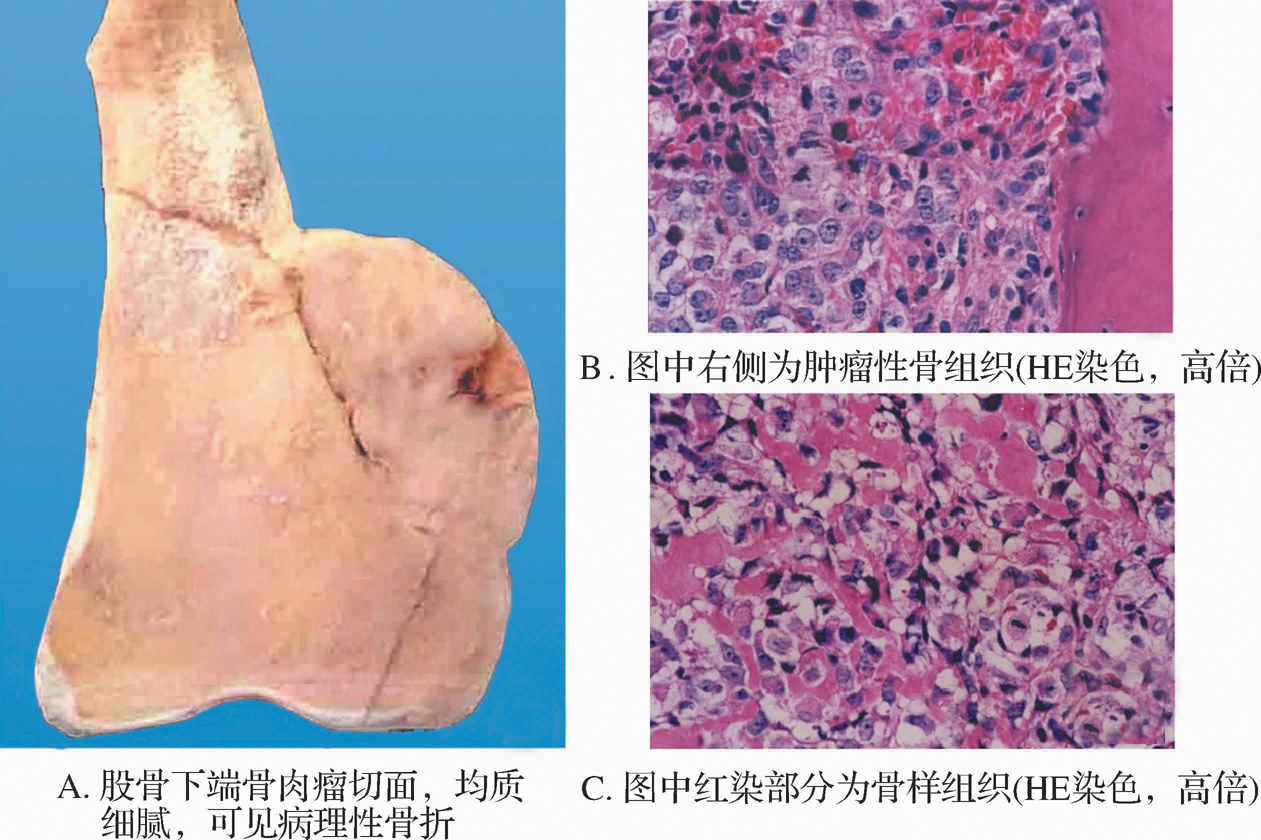
\includegraphics{./images/Image00086.jpg}
  \caption{骨肉瘤}
  \label{fig5-17}
\end{figure}

\subsection{神经组织肿瘤}

\subsubsection{周围神经组织肿瘤}

\paragraph{神经纤维瘤(neurofibroma)}
神经纤维瘤多发生在皮下,可单发也可多发。多发性神经纤维瘤又称神经纤维瘤病(neurofibromatosis)。肉眼观:单发者肿瘤境界明显,无包膜,质实,切面灰白色略透明,常不能找到其发源的神经。如发生肿瘤的神经粗大,则可见神经纤维消失于肿瘤中。镜下观:肿瘤由增生的神经鞘膜细胞和纤维母细胞构成,排列紧密,成小束并分散在神经纤维之间,伴多量网状纤维和胶原纤维及疏松的黏液样基质。神经纤维瘤较易复发,可恶变。

\paragraph{神经鞘瘤(neurilemmoma)}
神经鞘瘤可发生在周围神经、颅神经或交感神经。颅神经鞘瘤占颅内肿瘤的5%~10%,发生于听神经者,又称听神经瘤,位于小脑桥脑角。患者多为中老年,女多于男(2∶1)。肉眼观:神经鞘瘤有完整的包膜,呈圆形或结节状,常与其所发生的神经粘连在一起。切面为灰白或灰黄色略透明,可见旋涡状结构,有时还有出血和囊性变。镜下观:瘤细胞紧密平行排列呈栅状或不完全的漩涡状,或瘤细胞稀少排列成稀疏的网状结构。

临床表现随其大小与部位而异,小肿瘤可无症状,大多数肿瘤可手术根治,极少数与脑干或脊髓等紧密粘连未能完全切除者可复发,复发肿瘤仍属良性。

\subsubsection{中枢神经系统肿瘤}

中枢神经系统肿瘤无论组织分化程度如何,都可引起明显的临床症状,一方面肿瘤压迫或破坏周围组织引起局部神经症状,另一方面肿瘤可引起脑实质继发性充血、水肿,脑室积水扩张,导致颅内高压,产生相应症状,甚至危及生命。原发性中枢神经系统肿瘤以胶质瘤和脑膜瘤多见,胶质瘤中又以星形胶质细胞瘤多见。

\paragraph{星形胶质细胞瘤(astrocytoma)}
本瘤多见于成人,可发生于中枢神经系统的任何部位,但以大脑半球的白质最多见,儿童则多见于小脑。肉眼观:肿瘤无包膜,与周围脑组织并无明显分界,质地较硬,往往呈暗灰色胶冻样或细颗粒状。镜下观:瘤细胞的形态和分化程度可有很大差异,肿瘤细胞形态可相似于纤维型、原浆型或肥胖型星形胶质细胞,它们分别称为纤维型、原浆型和肥胖型星形胶质细胞瘤。高度恶性的星形胶质细胞瘤称为多形性胶质母细胞瘤。在临床实际工作中,根据星形胶质细胞瘤分化程度分为四级。一般而言,Ⅰ级的恶性程度较低,Ⅱ、Ⅲ、Ⅳ级的恶性程度逐渐增高。

\paragraph{脑膜瘤(meningioma)}
多数由蛛网膜颗粒中的蛛网膜细胞发生,一般生长缓慢。患者多为40~50岁中年人,女性较男性多。好发于上矢状窦旁大脑镰两侧、蝶骨嵴的侧面等处。肿瘤呈球形、分叶状或不规则形,质实或硬,边界清楚。切面灰白色,颗粒状或条索漩涡状,或有砂粒体(钙化物)形成。大多数脑膜瘤为良性,少数瘤组织可呈明显的异型性、浸润性生长和转移,称恶性脑膜瘤。

\subsection{多种组织构成的肿瘤}

畸胎瘤(teratoma)由三个胚层成分所构成的肿瘤,起源于有多向分化潜能的生殖细胞。好发于卵巢、睾丸、躯干中线及躯体两端,如颅底、松果体区、纵隔、腹膜后、骶尾等部位。本瘤根据肉眼观察分为囊性和实性畸胎瘤两种;根据分化程度分为成熟性(良性)和未成熟性(恶性)畸胎瘤。囊性者绝大多数为成熟性良性畸胎瘤;实性者多为未成熟性恶性畸胎瘤。

卵巢畸胎瘤多数是成熟性囊性畸胎瘤,约手拳大小,有包膜,囊腔内含黄色油脂样物质及毛发、牙齿等,囊壁可有增厚的结节状区域(图\ref{fig5-18})。镜下观:囊壁内衬多为复层鳞状上皮,有毛囊、皮脂腺等组织,故又称皮样囊肿。此外,亦可见软骨、支气管黏膜、胃肠黏膜或甲状腺组织等。肿瘤内所含的各种成分都可以发生恶变,但最常见的是鳞状上皮发生癌变。如杂有幼稚的神经管和神经上皮者也属于恶性。发生在睾丸的畸胎瘤多数为实性未成熟性,镜下见未成熟的胚胎性组织。未成熟性畸胎瘤属恶性畸胎瘤,可发生远处转移。

\begin{figure}[!htbp]
  \centering
  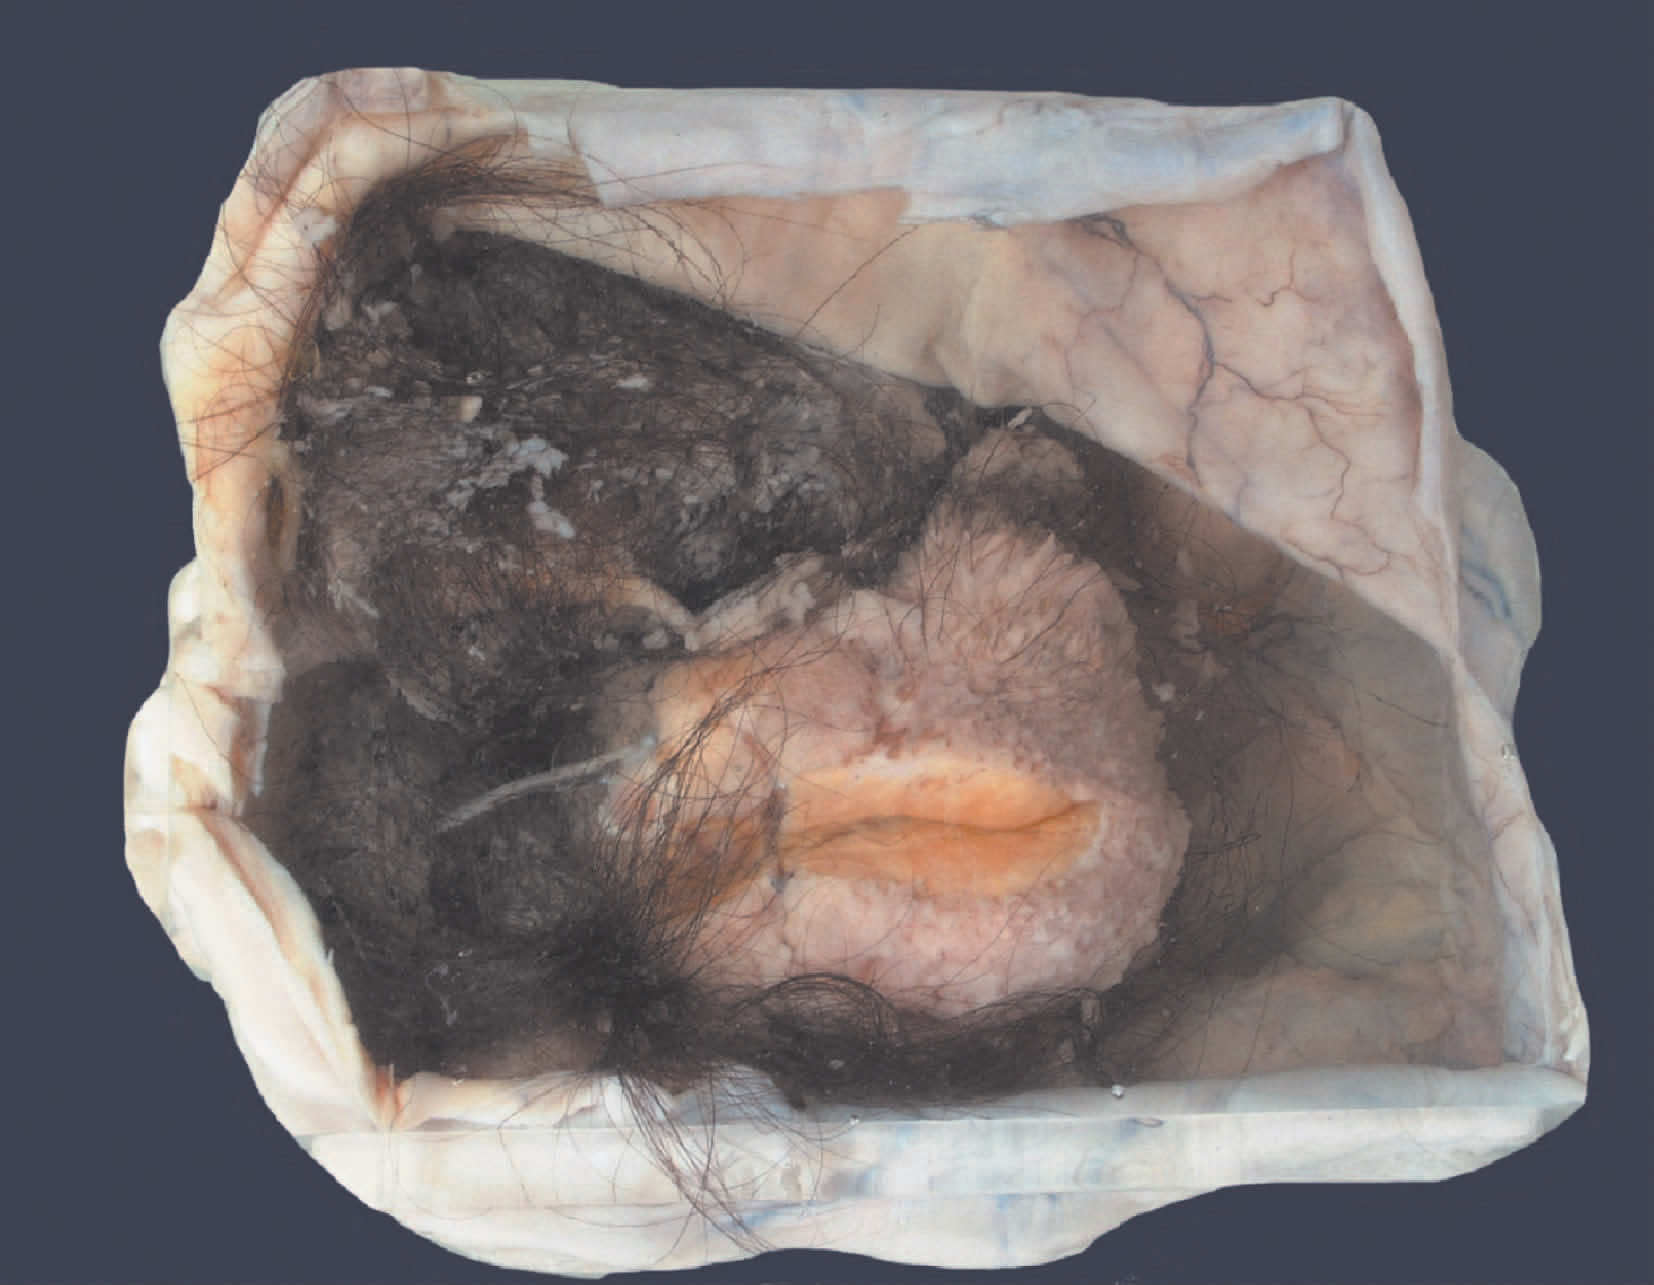
\includegraphics{./images/Image00087.jpg}
  \caption{卵巢囊性畸胎瘤}
  \label{fig5-18}
\end{figure}

\section{癌前病变、异型增生及原位癌}

因为中晚期恶性肿瘤治疗效果很差,所以肿瘤防治工作中一条重要的原则就是要做到三早(早期发现、早期诊断和早期治疗)。癌前病变和原位癌是肿瘤形成过程中非常重要的阶段,正确识别癌前病变和原位癌,并在这两个阶段进行早期治疗,具有非常重要的意义。

\subsection{癌前病变}

癌前病变(precancerous
lesion)是指一类具有癌变倾向,但不一定都会转变为癌的良性病变。癌前病变可能是肿瘤形成过程中的一个阶段,由于基因不稳定而具有潜在恶变的危险。在癌前病变恶变过程中,上述异型增生是非常重要的一个阶段。一般认为,正常细胞从增生发展到恶性肿瘤是个逐渐演变的过程:一般增生→异型增生→癌变。癌前病变出现异型增生则发生癌变的几率较大。

临床上常能观察到一些可能发生癌变的良性疾病,如黏膜白斑、慢性子宫颈炎、纤维囊性乳腺病、结肠多发性息肉病、慢性萎缩性胃炎、皮肤慢性溃疡、肝硬化、慢性胃溃疡等。临床上将这类具有癌变倾向的疾病列为癌前病变,然而有人主张应称之为癌前疾病或癌前状态,当这些病变中出现异型增生时,才能称之为癌前病变,进而可能癌变。

\subsection{异型增生}

异型增生(dysplasia),指细胞增生活跃,并伴一定程度异型性的病变,本身尚不具备癌的诊断标准。异型增生在组织学上表现为增生的细胞大小不一,形态多样;核大而深染,核浆比例增大,核分裂可增多,但多属正常核分裂像;细胞排列紊乱,极性消失。可发生于皮肤黏膜的被覆上皮,也可发生于腺上皮。根据其异型性程度及累及范围可分为轻、中、重三级。如发生在鳞状上皮,轻度异型增生累及上皮层下部1/3,中度累及下2/3,重度则超过下2/3但未及全层。轻度和中度异型增生,病因去除后多可恢复正常,重度异型增生较难逆转,常转变为癌。

\subsection{原位癌}

原位癌(carcinoma in
situ)是指局限于上皮层内,未突破基底膜侵犯到间质的恶性上皮性肿瘤(图\ref{fig5-19})。临床上可见于子宫颈、食管及皮肤的原位癌及乳腺小叶原位癌等。原位癌的诊断主要依赖于病理组织学。临床或肉眼检查往往无明显异常,或仅见有轻微糜烂、粗糙不平、局部增厚等。

\begin{figure}[!htbp]
  \centering
  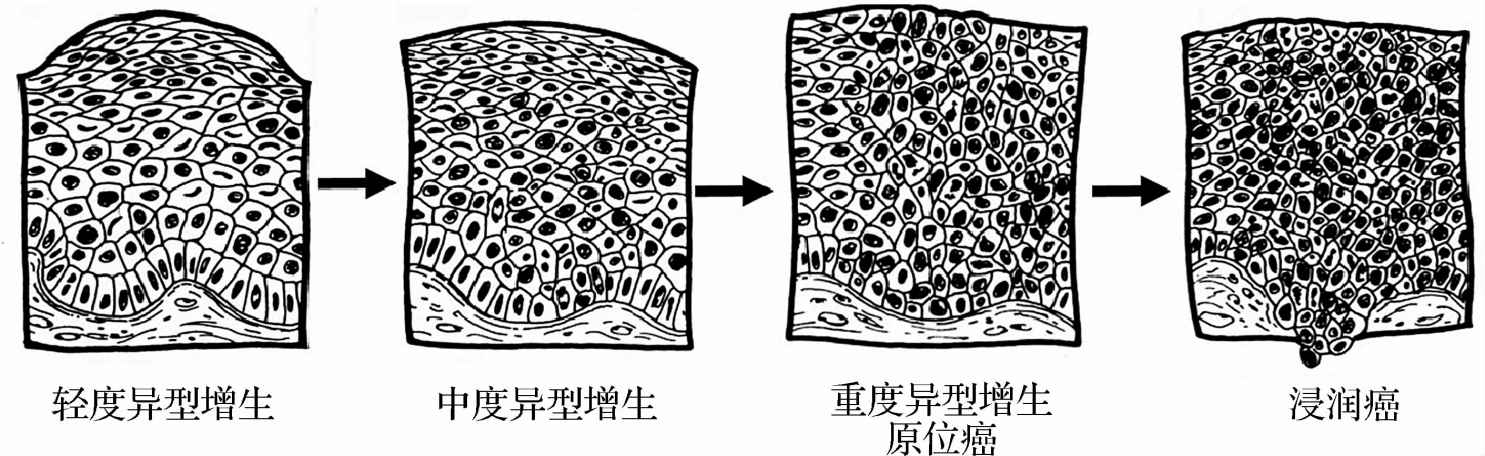
\includegraphics[width=0.7\textwidth]{./images/Image00088.jpg}
  \caption{异型增生、原位癌、早期浸润癌的演变过程模式图}
  \label{fig5-19}
\end{figure}

有少数原位癌可自行消退而恢复正常,或长期保持不变,也可数年后突破基底膜发展为浸润癌。由于上皮层内无血管、淋巴管,瘤细胞靠血液弥散获得营养,所以原位癌不发生转移。及时发现原位癌并给予治疗,可以完全治愈。

WHO最近提倡用“上皮内瘤变”(intraepithelial
neoplasia)的概念。将轻度和中度异型增生分别称为上皮内瘤变Ⅰ级和Ⅱ级,重度异型增生和原位癌称为上皮内瘤变Ⅲ级。例如:宫颈上皮内瘤变Ⅲ级。另外在胃肠道等上皮病变中,将轻度和中度异型增生称为低级别上皮内瘤变,而将重度异型增生和原位癌称为高级别上皮内瘤变。其用意可能是表达从异型增生到原位癌是一个连续的过程,无绝对界限,同时也表达了对原位癌的病人在术后无需进一步综合治疗,不给原位癌的病人戴上“癌”帽子的看法,这有利于患者。“上皮内瘤变”的概念被广泛应用于食管、子宫颈、前列腺等多个器官。

\section{肿瘤的病因及发病机制}

\subsection{肿瘤的病因}

肿瘤的病因甚为复杂,既包括外界环境中的各种刺激因素,也包括机体内在因素,而且往往是多因素交叉作用。一种致癌因素可通过不同途径引起不同部位的肿瘤,而同一类肿瘤又可由不同致癌因素引起。

\subsubsection{外环境致瘤因素}

\paragraph{化学性致瘤因素}
是最主要的致瘤因素。随着工业的迅速发展,将产生更多的化学性致瘤物质,污染环境,使一些癌肿发病率呈不断上升趋势,这一全球性问题已经引起高度重视。常见的化学性致瘤物质有:

(1)多环芳香烃类化合物:以3,4-苯并芘、1,2,5,6-双苯并蒽为代表广泛存在于煤烟、沥青、内燃机废气、烟草烟雾中,人工合成的如3-甲基胆蒽等。这些致癌物经体内代谢活化后可致癌。

(2)芳香胺类及氨基偶氮染料:如奶油黄、猩红等可引起大鼠实验性肝癌。印染厂空气中的乙萘胺,在体内代谢转变为氨基苯,由肾脏经膀胱排出,可致膀胱癌。

(3)亚硝胺类:该类化合物广泛存在于自然界,具有强烈的致癌作用。其前身物亚硝酸盐及二级胺可在胃内酸性环境下形成亚硝胺,致癌谱很广,可引起胃肠道及其他部位肿瘤。不同结构的亚硝胺有不同的器官亲和性,而与给药途径无关。亚硝胺类是间接作用的化学致癌物,在体内经羟化作用活化后,具有致癌作用。

(4)真菌毒素:某些真菌毒素有强烈的致癌作用,如黄曲霉毒素。黄曲霉毒素主要存在于霉变的花生、玉米及谷类中,其中以黄曲霉毒素B{1}
致癌性最强,与人肝癌的发生有关,动物实验中能诱发大鼠肝癌,其作用环节为黄曲霉毒素在内质网内氧化成环氧化物与DNA结合致癌。

(5)微量元素:对人类有致癌性的微量元素有砷、镍、铬、镉等。砷、铬、镍与肺癌的发生有关,镉可引起前列腺癌,钼或硒的缺乏与肿瘤的发生有一定关系。

(6)其他:在塑料工业中广泛应用的氯乙烯,可诱发大鼠肺、骨及皮肤等处的肿瘤,也可引起人的肝血管肉瘤。

\paragraph{物理性致瘤因素}
包括电离辐射(X线、放射性同位素)、紫外线、热辐射、异物(片状异物、石棉纤维)等。如原子弹爆炸的电离辐射使受染区人群白血病发病率明显增高,过量紫外线照射可致皮肤癌,石棉纤维可致胸膜恶性间皮瘤。物理性致瘤因素多与损伤染色体有关,其致瘤所需时间长,肿瘤发生率相对较低。由于致瘤因素较明确,防护措施较易奏效。

\paragraph{生物性致瘤因素}
(1)病毒:自从20世纪初发现鸡白血病可用无细胞滤液传递以来,现已知有600多种动物的致瘤病毒,其中1/3为DNA病毒,2/3为RNA病毒,前者如乳头状瘤病毒、多瘤病毒、空泡病毒、腺病毒、疱疹病毒等,后者如人类T细胞白血病/淋巴瘤病毒Ⅰ(HTLV-1)。

科学家对人类肿瘤的病毒致瘤问题进行了深入研究,发现人的白血病、乳腺癌、鼻咽癌、子宫颈癌、霍奇金病等肿瘤细胞内查见有“病毒颗粒”;鼻咽癌、子宫颈癌患者血清中有特异性抗病毒抗体;HTLV-1与人T细胞白血病/淋巴瘤有关;人类乳头状瘤病毒(HPV)与人子宫颈和肛门生殖器区域的鳞状细胞癌有关;Epstein-Barr病毒(EBV)与人的伯基特淋巴瘤和鼻咽癌有关;乙肝病毒(HBV)与肝细胞癌的发生有密切关系。但迄今为止,这些病毒既不能使正常细胞转化,也未能在动物中诱发肿瘤,因此病毒在人类肿瘤发病中的作用须进一步研究。

(2)细菌:幽门螺杆菌(H.
pylori)为革兰阴性杆菌,是慢性胃炎和胃溃疡的重要病原因素。幽门螺杆菌感染与胃的黏膜相关组织(mucosa-associated
lymphoid
tissue,MALT)发生的MALT淋巴瘤密切相关。幽门螺杆菌胃炎与一些胃腺癌的发生也有关系,特别是局限于胃窦和幽门的幽门螺杆菌感染。

{ \subsubsection{影响肿瘤发生发展的内因} }

\paragraph{遗传因素}
动物实验中发现在同一外界致瘤因素刺激下,不同基因型的动物发病率不同。人类某些肿瘤有明显家族遗传倾向。如结肠多发性息肉、视网膜母细胞瘤、神经纤维瘤、肾母细胞瘤等。也有一些患者有肿瘤家族史,父母兄妹中易患肿瘤,但肿瘤类型可各不相同。肿瘤家族史或遗传因素在肿瘤发病中仅是一种“易感性”,作为环境致癌因素作用的基础。

\paragraph{年龄因素}
某些肿瘤的发生有一定的年龄分布,如儿童易患急性白血病、肾母细胞瘤等。青年人则以骨肉瘤、横纹肌肉瘤多见。40岁以上中老年则癌的发病率增高。幼儿和儿童的肿瘤,常与遗传性基因缺陷有关,老年人癌肿发病率高的原因可能与某些致癌物质长期积累,引起体细胞突变及免疫机能下降有关。

\paragraph{内分泌因素}
某些肿瘤的发生与内分泌激素的刺激有密切关系,如雌激素过高与乳腺癌、子宫内膜癌的发生、发展有关,切除卵巢对乳腺癌有治疗作用。某些激素与肿瘤浸润、转移有关,如垂体前叶激素可促进肿瘤的生长和转移,而肾上腺皮质激素则对淋巴造血系统肿瘤的生长和转移有抑制作用。

\paragraph{免疫因素}
实验和临床观察均证明,肿瘤的发生发展、疗效和预后都与机体的免疫状态有关。动物实验发现,无胸腺、无脾脏的裸鼠诱癌的敏感性明显高于正常小鼠;先天性免疫缺陷或后天免疫缺陷如器官移植术后大量应用免疫抑制剂的患者,恶性肿瘤的发生率,特别是淋巴瘤的发生率明显增高。

肿瘤抗原引起的宿主免疫反应主要是细胞免疫。四种免疫细胞在肿瘤免疫中起重要作用:T细胞,尤其是T杀伤细胞,可释放淋巴因子和溶解酶杀伤肿瘤细胞;自然杀伤细胞(NK)无需预先致敏,可直接杀伤肿瘤细胞;K细胞在淋巴细胞依赖性抗体的参与下对癌细胞起杀伤作用(ADCC);巨噬细胞在淋巴因子如白细胞介素-2、巨噬细胞活化因子等作用下聚集到肿瘤周围,并在嗜细胞抗体协同下,杀伤肿瘤细胞。体液免疫在破坏溶解肿瘤细胞中也有一定作用。

肿瘤可破坏宿主免疫机能,保护肿瘤细胞免受宿主攻击,使肿瘤继续生长和转移,这种现象称为“免疫逃逸”。根据肿瘤与宿主相互作用的免疫机制,临床上对肿瘤患者作免疫功能检测,对病人预后的估计有重要参考价值。现代免疫治疗的发展,成为肿瘤综合治疗的重要组成部分。

\subsection{肿瘤的发病机制}

\subsubsection{正常细胞的癌变}

肿瘤的发生是细胞生长异常,分化失控的结果。正常细胞转变为癌细胞首先要经过转化阶段,形成转化细胞,表现为染色体畸变,核大深染,增殖加快,并产生某些新的肿瘤抗原。这种细胞能进一步形成肿瘤,也可能死亡或恢复正常。目前认为下面几种分子的结构或功能异常是肿瘤发生的重要分子基础。

\paragraph{癌基因(oncogene)}
正常细胞或病毒中存在一类基因,具有高度进化保守性和重要的生理功能,参与胚胎发育、细胞增殖和分化调控等。在正常情况下,该类基因不表达或表达水平较低,没有致癌性,称为原癌基因或细胞癌基因。在致癌因素作用下,原癌基因被激活,诱导细胞恶变,此时即称之为癌基因。激活的途径包括点突变、染色体重排(图\ref{fig5-20})和基因扩增等。癌基因的产物有生长因子及其受体、信号转导分子、转录因子、细胞周期调控蛋白等,这些产物增加即促进细胞增殖(图\ref{fig5-21})。目前发现的癌基因颇多,重要的如ras、myc、sis等。

\begin{figure}[!htbp]
  \centering
  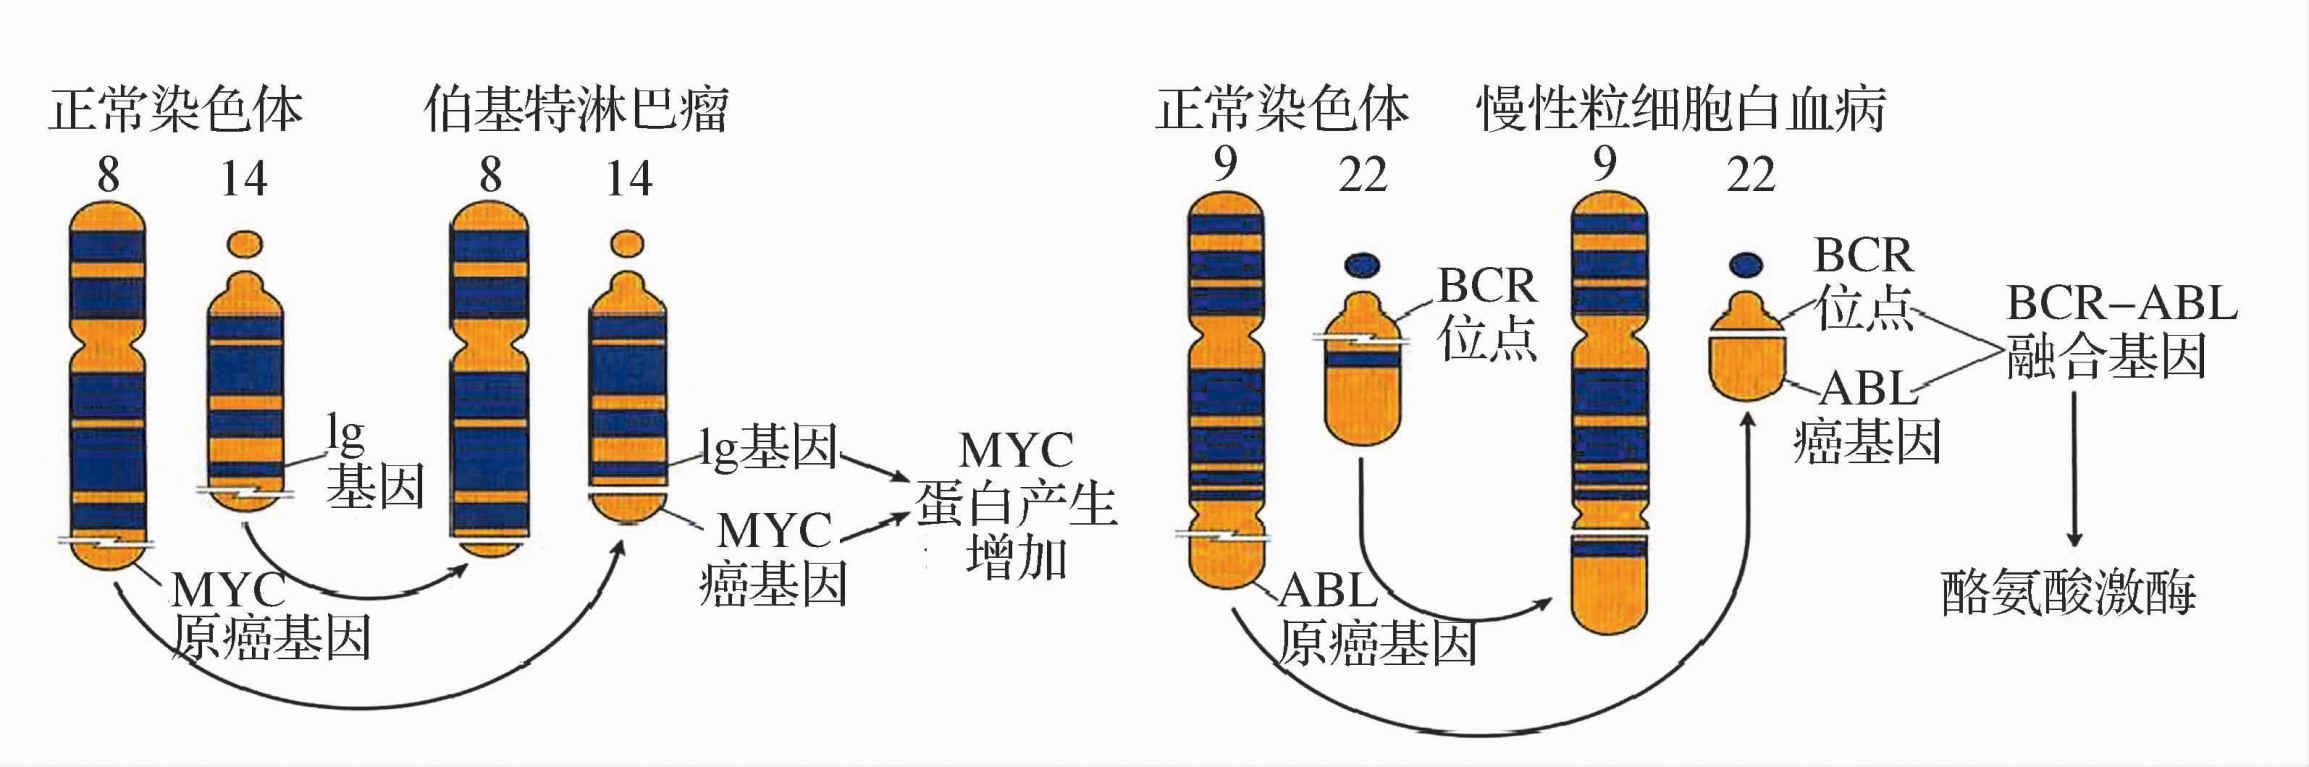
\includegraphics[scale=1.2]{./images/Image00089.jpg}
  \caption{染色体重排与肿瘤发生的关系}
  \label{fig5-20}
\end{figure}

\begin{figure}[!htbp]
  \centering
  
\includegraphics{./images/Image00090.jpg}
  \caption{原癌基因激活的后果}
  \label{fig5-21}
\end{figure}

\paragraph{肿瘤抑制基因}
是正常细胞中存在的一类对细胞增殖起负调节作用的基因,这类基因产物直接或间接地抑制细胞增生和肿瘤性转化,故又称为抑癌基因(anti-oncogene)。抑癌基因的失活或突变均可引起细胞癌变、浸润或转移等。目前已发现多种抑癌基因,如乳腺癌、白血病、低分化结肠癌等肿瘤中的p53基因(图\ref{fig5-22}),视网膜母细胞瘤、骨肉瘤中的Rb基因和肺癌、胰腺癌中的p16,结肠腺瘤性息肉病的APC基因,神经纤维瘤病的NF-1基因等。

\begin{figure}[!htbp]
  \centering
  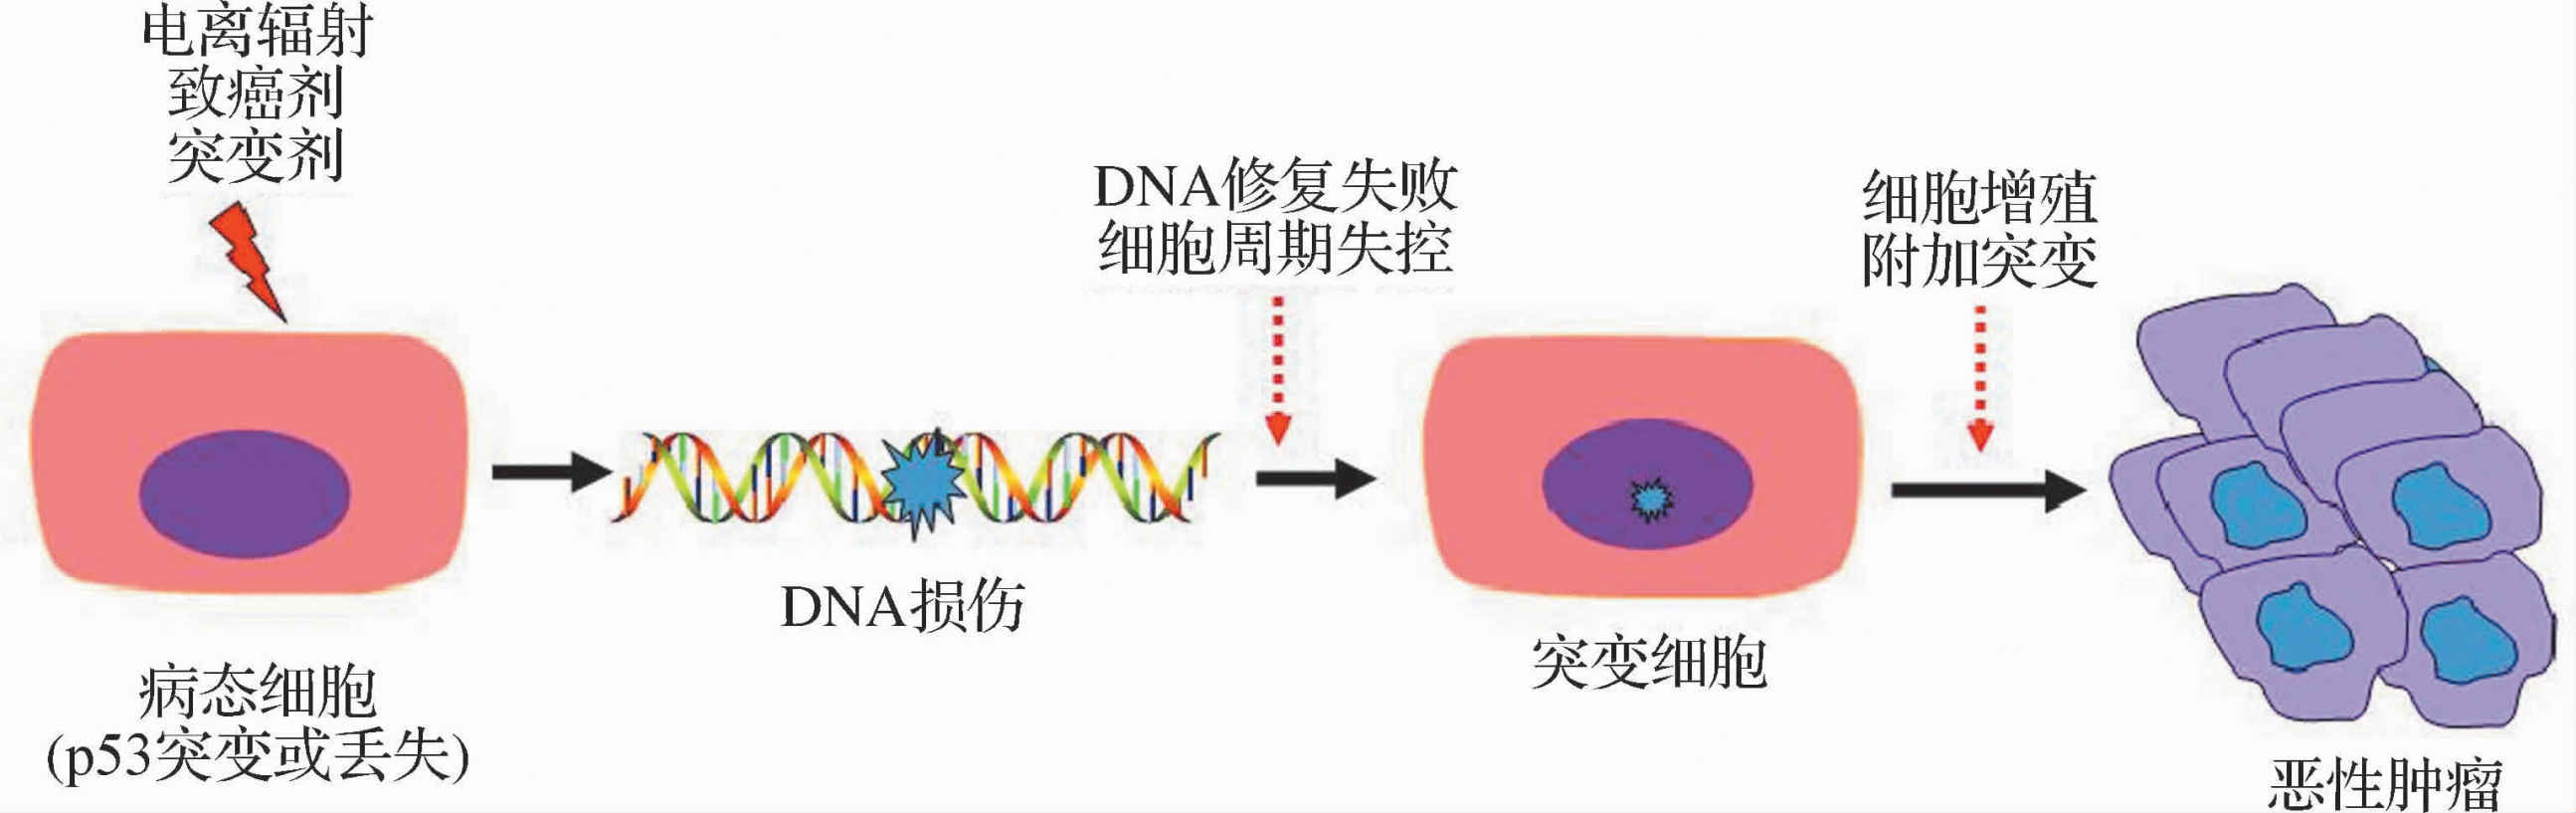
\includegraphics[scale=1.1]{./images/Image00091.jpg}
  \caption{p53基因突变或丢失的后果}
  \label{fig5-22}
\end{figure}

恶性肿瘤的发生是一个长期的、多因素造成的分阶段的过程。单个基因的改变不能造成细胞的完全恶性转化,大多数肿瘤的发生需要几个癌基因的激活和抑癌基因的丧失或突变。

\paragraph{凋亡调节基因和DNA修复调节基因}
除了原癌基因的激活与肿瘤抑制基因的失活外,近年来还发现调节细胞进入凋亡或程序性细胞死亡(programmed
cell
death,PCD)的基因及其产物在某些肿瘤的发生上也起着重要作用。如Bcl(B-cell
lymphoma/1eukemia)家族中的Bcl-2蛋白可以抑制凋亡,而Bax蛋白则可以促进细胞凋亡。正常情况下Bcl-2和Bax在细胞内保持平衡。如Bcl-2蛋白增多,细胞则长期存活;如Bax蛋白增多,细胞则进入凋亡。

人类在生活中接触到许多致癌物,如电离辐射、化学物质等。这些致癌物引起的DNA损害如果超过细胞能够忍受的范围,受损细胞会以凋亡的形式死亡;如果引起轻微的DNA损害,正常细胞内的DNA修复机制可及时进行修复。这对维持机体遗传基因组的稳定非常重要。在一些有遗传性DNA修复调节基因突变或缺陷的人中,肿瘤的发病率极高。

\paragraph{端粒、端粒酶和肿瘤}
正常细胞分裂一定次数后就进入老化阶段,失去了复制的能力,称为复制老化。近来的研究已证明细胞的复制次数是由一种位于染色体末端的叫做端粒(telomere)的特殊DNA重复序列控制的,端粒对保持染色体稳定具重要作用。随细胞DNA复制次数增加而逐渐缩短,故又称生命计时器。在染色体末端的端粒酶(telomerase)能通过逆转录作用不断合成缩短的序列,从而维持端粒长度,维持细胞增殖潜能。大多数体细胞不含端粒酶,大多恶性肿瘤细胞端粒酶活性上调。

\paragraph{表观遗传调控与肿瘤}
表观遗传调控是一种不涉及DNA碱基序列改变的基因表达调控方式。常通过DNA甲基化、组蛋白乙酰化等途径进行调节。微小RNA(microRNA)和长链非编码RNA(lncRNA)为近年发现的表观遗传调控新成员,它们不编码蛋白质,但对基因表达有直接或间接影响。

\subsubsection{肿瘤发生的过程}

目前经病理学、分子生物学、遗传学和流行病学等多方面的研究表明,肿瘤的发生是一个多步骤多基因改变共同作用的过程。例如,目前已知结肠的上皮增生、异型增生、腺瘤到最终形成腺癌的过程中包括APC抑癌基因失活、ras基因的活化、18号染色体长臂上Smad2基因和Smad4基因的丢失,最后p53和TGF-β受体Ⅱ基因的失活。

综上所述,环境因素及遗传因素等导致细胞DNA发生突变,细胞的进一步恶性转化涉及癌基因的激活和抑癌基因的失活及凋亡调节基因和DNA修复基因的异常改变导致瘤细胞单克隆增殖,并进一步发生肿瘤细胞的异质化,形成恶性肿瘤(图\ref{fig5-23})。

\begin{figure}[!htbp]
  \centering
  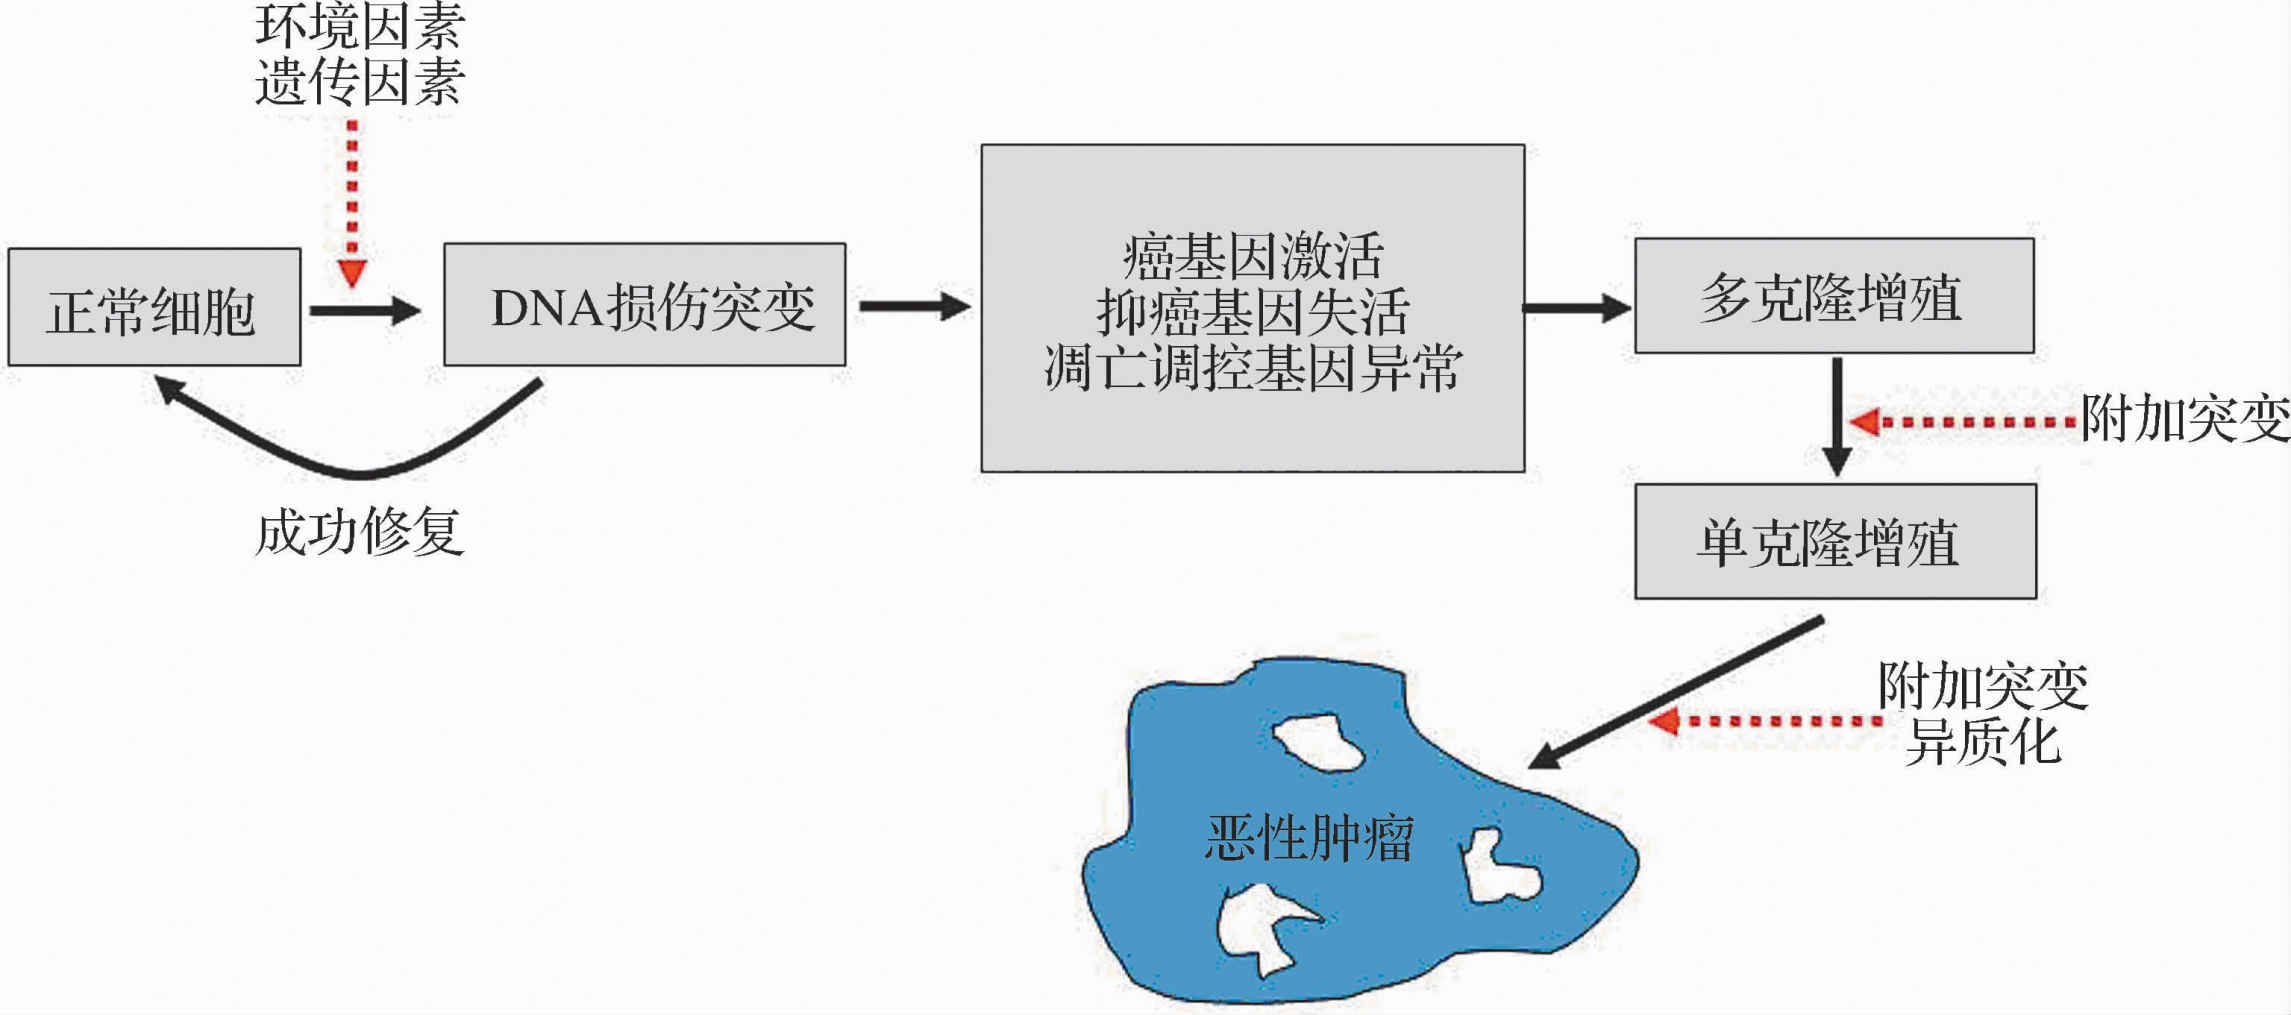
\includegraphics[scale=1.2]{./images/Image00092.jpg}
  \caption{恶性肿瘤发生示意图}
  \label{fig5-23}
\end{figure}

\section*{复习与思考}

{一、名词解释}

肿瘤的实质 异型性 直接蔓延 转移 种植性转移 癌 肉瘤 癌前病变 胶样癌
畸胎瘤 交界性肿瘤 恶病质 异型增生 原位癌 癌基因 抑癌基因

{二、问答题}

1. 肿瘤性增生与炎症、损伤修复时组织增生有何不同?

2. 列表比较良性肿瘤与恶性肿瘤的区别。

3. 何谓异型增生和原位癌?

4. 常见上皮性恶性肿瘤有哪些?各有何特征?

5. 简述肿瘤的组织结构。

6. 何谓肿瘤异型性?其形态表现如何?

7. 何谓肿瘤转移?转移方式有几种?

8. 癌与肉瘤有何区别?

9. 简述肿瘤的命名原则。

10. 什么叫癌前疾病?常见的癌前疾病有哪几种?

11. 肿瘤的生长方式有哪几种?肿瘤生长方式与肿瘤的良性、恶性有何关系?

12. 试述良性、恶性肿瘤对机体的影响。

13. 常见上皮性良性肿瘤有哪些?各有何特征?

14. 常见上皮性恶性肿瘤可分哪几类?各有何特征?

{三、临床病理分析}

病史摘要:男性,75岁,上腹部隐痛4年余,去年起腹痛加剧,经常呕吐。两个月来,面部及手足水肿,尤以左上肢为显著,尿量减少,食欲极差。半小时前,排黑色大便,呕吐大量鲜血,突然昏倒而急诊入院。体检:消瘦,面色苍白,四肢厥冷,血压60/40
mmHg,心音快而弱。两侧颈部、左锁骨上及腋下淋巴结显著肿大,血红蛋白60
g/L。血浆总蛋白42 g/L,白蛋白14 g/L。抢救无效死亡。

尸检所见:发育尚好,体形消瘦,营养较差,下肢有轻度凹陷性水肿。左锁骨上淋巴结肿大约枣子大小,粘连。右侧胸腔积液约400
ml。腹部膨隆,腹腔内有黄色半混浊液体4 000
ml,大网膜和胃壁粘连,表面有灰白大小不等结节多个。胃内容物为咖啡渣样液体,窦部小弯侧有5
cm直径的溃疡一个,边缘呈围堤状隆起,底部见一小凝血块。肝、肺表面有灰白小结节。左锁骨上淋巴结灰白色、肿大。胃溃疡取材镜检:瘤细胞以立方形为主,呈条索或团块状,偶见腺样结构形成。肿瘤细胞异型性明显,细胞核大小、形态不一,核分裂像多见。少数瘤细胞核偏位,胞质中含有黏液颗粒。瘤组织和周围正常组织分界不清,累及胃壁全层。其他脏器病变组织学检查与胃相似。

讨论题:

1. 胃及其他器官病变的病理诊断是什么?

2. 试述各脏器病变的发生发展关系。

3. 试述上述病变的临床和病理联系。

4. 分析病人的死亡原因。




